%% Hey gutter! Jeg håber I er færdige nu, ellers venter I bare med at svare til i er :heart:
%%
%% I forhold til oplæsning er følgende min plan:
%% Jeg præsenterer alle emnerne, så I ikke behøver lave andet end at læse op. Hvis nogen har lyst til at præsentere må de selvfølgelig også det, men jeg har ingen andre kurser, så det er absolut oplagt for mig at gøre det. Hvis I gerne vil, men ikke har tid til at lave slides, kan I bare bruge mine. Jeg skal bare lige give jer adgang til mine noter på github. Jeg skal nok få lavet nogle gode kahoots til dem alle den her gang ;)
%% 17. Maj:
%%    Spørgsmål 1
%% Pensum:
%% * (Sipser 1.1-1.3)
%% * Sipser 1.4: \textbf{Non-regular Languages}
%% * Sipser 2.3: \textbf{Non-context-free Languages}
%% * Weekly Note 1
%% * Video 1
%% * Video 2
%%
%% 19. Maj:
%%    Spørgsmål 2
%% Pensum:
%% * Sipser 2.1-2.2: \textbf{Pushdown Automata and Context-free Languages}
%% * Weekly Note 2
%% * Video 3-6
%%
%% 21. Maj:
%%    Spørgsmål 3
%% Pensum:
%% * Sipser 3: \textbf{Turing Machines}
%% * Weekly Note 3
%% * Weekly Note 4
%% * Video 7-10
%%
%% 23. Maj:
%%    Spørgsmål 4
%% Pensum:
%% * Sipser 4: \textbf{Afgørlighed} (Undtagen Sætning 4.17)
%% * Siper 5.1 pp. 215-220 + 5.3: \textbf{Reducérbarhed}
%% * Weekly Note 5
%% * Weekly Note 6
%% * Video 11-14
%%
%% 25. Maj:
%%    Spørgsmål 5
%% Pensum:
%% * Siper 7.1-7.4: \textbf{Tidskompleksitet inkl. P, NP, NP-komplethed}
%% * CLRS 34: \textbf{NP-Komplethed Beviser} (minus sider 1070-1078)
%% * Weekly Note 7
%% * Weekly Note 8
%% * Weekly Note 9 (ish)
%% * Video 15-17
%%
%% 27. Maj:
%%    Spørgsmål 6
%% Pensum:
%% * Sipser 7.4: \textbf{Bevis at CNF-SAT er NP-Komplet}
%% * Weekly Note 9
%% * Video 18 (Bonus \href{https://www.youtube.com/watch?v=6Az1gtDRaAU}{video})
%%
%% 29. Maj:
%%    Spørgsmål 7
%% Pensum:
%% * CLRS 35: \textbf{Approximationsalgoritmer}
%% * Weekly Note 10 (igen)
%% * Video 19-21
%%
%% 31. Maj:
%%    Spørgsmål 8
%% Pensum:
%% * Baase 2.4: \textbf{Informationsteoretiske nedre grænser for sortering ved sammenligninger}
%% * Jørgens noter: \textbf{Noter på nedre grænser}
%% * CLRS 9.3: \textbf{Median Problem}
%% * Weekly Note 11
%% * Video 22-24
%%
%% 2. Juni:
%%    Spørgsmål 9
%% Pensum:
%% * Baase 3: \textbf{Adversary nedre grænse argumenter}
%% * Baase 3.5: \textbf{Adversary Median Problem}
%% * Jørgens noter: \textbf{Noter på nedre grænser}
%% * Weekly Note 12
%% * Video 24-25
%%
%% 4. Juni:
%%    Spørgsmål 10
%% Pensum:
%% * Cygan et al pp. 3-8, 12-14, 17--22, 51-55: \textbf{Algoritmer med faste parametre}.
%% * F.V. Fomin, D. Kratsch pp. 1-6: \textbf{Eksakte Algoritmer}.
%% * Weekly Note 13
%% * Video 26
%%
%% 5-12 juni: (8 dage inkl.)
%% Se på de svage led, øvepræsentationer, muligvis opgaver

% !TEX TS-program = xelatex
% !TEX encoding = UTF-8 Unicode
\documentclass[12pt, oneside, a4paper]{book}

\usepackage[top=3cm, bottom=3cm, left=3cm, left=3cm, right=3cm, headsep=10pt,a4paper]{geometry}


\usepackage{sourcesanspro}
\usepackage{tgpagella}

\usepackage[utf8]{inputenc} % Tillader utf-8 kodning
\usepackage[T1]{fontenc} % Kodning der fungerer bedre til europæiske sprog
\usepackage{microtype}

\usepackage{float} % Tillader [H]

\usepackage{wrapfig} % Alignment til figurer



% Sæt sproget til dansk
\usepackage{polyglossia}
\setdefaultlanguage{danish}
\setotherlanguages{english}

% Til ordbogen
\usepackage{longtable}

% For bedre tabeller
\usepackage{multirow}


% So that file names with multiple dots don't confuse
% graphicx package when using \includegraphics command:
\usepackage[multidot]{grffile}
\usepackage{graphicx}

\usepackage{xcolor}
\usepackage{amsmath, amsfonts, mathtools, amsthm, amssymb}


\usepackage{tikz} % Til grafer
\usetikzlibrary{automata} % Til automatgrafer
\usetikzlibrary{positioning} % Positionering af knuder
\usetikzlibrary{arrows.meta, arrows} % arrows til at ændre kanter
\tikzset{
	node distance=2.5cm, % minimumsdistancen mellem to knuderj
	every state/.style={
			semithick,
			fill=gray!10
		},
	initial text={}, % Ingen tekst, bare kanter
	double distance=2pt, % Udseende på accept states
	every edge/.style={ % Egenskaber for hver transition
			draw,
			>=stealth', % bold arrowheads
			auto,
			semithick
		}
}
% Tak til: https://www3.nd.edu/~dchiang/teaching/theory/2018/www/tikz_tutorial.pdf





\usepackage{enumerate} % allows customized labels in enumerations
\usepackage{hyperref}  % makes cross references and URLs clickable


% Til at customize titler
\usepackage{titlesec}

% Til algoritmer
\usepackage{algorithm}
\usepackage{algorithmic}

\renewcommand{\algorithmicrequire}{\textbf{Kræver}}
\renewcommand{\algorithmicensure}{\textbf{Sikrer}}
\renewcommand{\algorithmicif}{\textbf{hvis}}
\renewcommand{\algorithmicthen}{\textbf{s\aa}}
\renewcommand{\algorithmicelse}{\textbf{ellers}}
\renewcommand{\algorithmicfor}{\textbf{for}}
\renewcommand{\algorithmicforall}{\textbf{for alle}}
\renewcommand{\algorithmicdo}{\textbf{gør}}
\renewcommand{\algorithmicwhile}{\textbf{mens}}
\renewcommand{\algorithmicrepeat}{\textbf{gentag}}
\renewcommand{\algorithmicuntil}{\textbf{indtil}}
\renewcommand{\algorithmicreturn}{\textbf{returner}}
\renewcommand{\algorithmiccomment}[1]{\hfill\textit{#1}}

% Colors
\definecolor{DeepSeaBlue}{HTML}{264653}
\definecolor{TurquoiseGreen}{HTML}{2a9d8f}
\definecolor{SunnyYellow}{HTML}{e9c46a}
\definecolor{SunsetOrange}{HTML}{f4a261}
\definecolor{CoralRed}{HTML}{e76f51}
\definecolor{Light}{HTML}{686868}
\definecolor{Steel}{HTML}{888888}
\definecolor{Dark}{HTML}{262626}

\definecolor{DeepSeaBlueLighter}{HTML}{2d5363}
\definecolor{DeepSeaBlueDarker}{HTML}{1e3742}
\definecolor{DeepSeaBlueMuted}{HTML}{2c434c}

\definecolor{TurquoiseGreenLighter}{HTML}{32bcab}
\definecolor{TurquoiseGreenDarker}{HTML}{217d72}
\definecolor{TurquoiseGreenMuted}{HTML}{3b8b81}

\definecolor{SunnyYellowLighter}{HTML}{f1dba5}
\definecolor{SunnyYellowDarker}{HTML}{e0ac2e}
\definecolor{SunnyYellowMuted}{HTML}{d5bc7d}

\definecolor{SunsetOrangeLighter}{HTML}{f8c7a0}
\definecolor{SunsetOrangeDarker}{HTML}{ef7c21}
\definecolor{SunsetOrangeMuted}{HTML}{dda477}

\definecolor{CoralRedLighter}{HTML}{ee9c87}
\definecolor{CoralRedDarker}{HTML}{db441e}
\definecolor{CoralRedMuted}{HTML}{d07c67}

\hypersetup{
	pdfauthor={Kevin Vinther},
	pdftitle={DM553 Noter},
	pdfsubject={computer science, complexity, computability},
	colorlinks=true,
	linkcolor=DeepSeaBlue,
	urlcolor=DeepSeaBlue,
}

% Define color for headings
\definecolor{HeadingColor}{HTML}{264653}

% Chapter title formatting
\titleformat{\chapter}[block] % 'block' for inline display
  {\normalfont\sffamily\huge\bfseries\color{HeadingColor}} % Chapter title styling
  {\thechapter. } % Prefix for the title, such as "1. "
  {0pt} % Space between the number and title
  {} % Additional formatting for the title

% Section title formatting
\titleformat{\section}
  {\normalfont\sffamily\Large\bfseries\color{HeadingColor}}
  {\thesection} % Section number
  {1em} % Space between number and section title
  {}

% Subsection title formatting
\titleformat{\subsection}
  {\normalfont\sffamily\large\bfseries\color{HeadingColor}}
  {\thesubsection} % Subsection number
  {1em} % Space between number and subsection title
  {}

% Subsubsection title formatting
\titleformat{\subsubsection}
  {\normalfont\sffamily\normalsize\bfseries\color{HeadingColor}}
  {\thesubsubsection} % Subsubsection number
  {1em} % Space between number and subsubsection title
  {}

% For subsubsections, if needed, you can define a \paragraph formatting
\titleformat{\paragraph}[runin]
  {\normalfont\sffamily\normalsize\bfseries\color{HeadingColor}}
  {\theparagraph} % Paragraph number
  {1em} % Space between number and paragraph title
  {}

% Adjust spacing around sectional units
\titlespacing*{\chapter}{0pt}{50pt}{40pt}
\titlespacing*{\section}{0pt}{20pt}{10pt}
\titlespacing*{\subsection}{0pt}{15pt}{10pt}
\titlespacing*{\subsubsection}{0pt}{10pt}{5pt}
\titlespacing*{\paragraph}{0pt}{10pt}{5pt}


\setcounter{secnumdepth}{3}
\setcounter{tocdepth}{3}




% Now apply the custom style
\theoremstyle{customstyle}


% Pænere teoremdefinitioner, etc.
% theorems
\usepackage{thmtools}
\usepackage[framemethod=TikZ]{mdframed}

\mdfsetup{skipabove=1em,skipbelow=0em}

\newcounter{mycounter}
\numberwithin{mycounter}{chapter}

\newcounter{notecounter}
\numberwithin{notecounter}{chapter}

% Green Box
\declaretheoremstyle[
    headfont=\bfseries\sffamily\color{TurquoiseGreen!70!black},
    notefont=\bfseries\sffamily\color{TurquoiseGreen!70!black}, % same style for the note
    notebraces={}{}, % to remove parentheses around the note
    bodyfont=\normalfont,
    postheadspace=\newline, % adds a new line after the theorem head
    headformat={\NAME\ \NUMBER\ \NOTE \vspace{0.2cm}}, % Custom head format
    mdframed={
        linewidth=2pt,
        rightline=false, topline=false, bottomline=false,
        linecolor=TurquoiseGreen, backgroundcolor=TurquoiseGreen!5,
        nobreak=false,
		innerbottommargin=10pt, % Adjust the inner bottom margin within the frame
    skipbelow=10pt,         % Adjust the space after the frame
    }
]{thmgreenbox}

% Red Box
\declaretheoremstyle[
    headfont=\bfseries\sffamily\color{CoralRed!70!black},
    notefont=\bfseries\sffamily\color{CoralRed!70!black}, % same style for the note
    notebraces={}{}, % to remove parentheses around the note
    bodyfont=\normalfont,
    postheadspace=\newline, % adds a new line after the theorem head
    headformat={\NAME\ \NUMBER\ \NOTE \vspace{0.2cm}}, % Custom head format
    mdframed={
        linewidth=2pt,
        rightline=false, topline=false, bottomline=false,
        linecolor=CoralRed, backgroundcolor=CoralRed!5,
        nobreak=false,
		innerbottommargin=10pt, % Adjust the inner bottom margin within the frame
    skipbelow=10pt,         % Adjust the space after the frame
    }
]{thmredbox}

% Blue Box
\declaretheoremstyle[
    headfont=\bfseries\sffamily\color{DeepSeaBlue!70!black},
    notefont=\bfseries\sffamily\color{DeepSeaBlue!70!black}, % same style for the note
    notebraces={}{}, % to remove parentheses around the note
    bodyfont=\normalfont,
    postheadspace=\newline, % adds a new line after the theorem head
    headformat={\NAME\ \NUMBER\ \NOTE \vspace{0.2cm}}, % Custom head format
    mdframed={
        linewidth=2pt,
        rightline=false, topline=false, bottomline=false,
        linecolor=DeepSeaBlue, backgroundcolor=DeepSeaBlue!5,
        nobreak=false,
		innerbottommargin=10pt, % Adjust the inner bottom margin within the frame
    skipbelow=10pt,         % Adjust the space after the frame
    }
]{thmbluebox}

\declaretheorem[style=thmredbox, name=Sætning, numberlike=mycounter]{theorem}
\declaretheorem[style=thmgreenbox, name=Definition, numberlike=mycounter]{definition}
\declaretheorem[style=thmredbox, name=Lemma, numberlike=mycounter]{lemma}
\declaretheorem[style=thmredbox, name=Proposition, numberlike=mycounter]{proposition}
\declaretheorem[style=thmredbox, name=Corollary, numberlike=mycounter]{corollary}
\declaretheorem[style=thmredbox, name=Formodning, numberlike=mycounter]{conjecture}
\declaretheorem[style=thmbluebox, name=Påstand, numberlike=mycounter]{claim}
\declaretheorem[style=thmbluebox, name=Eksempel, numberlike=mycounter]{example}
\declaretheorem[style=thmbluebox, name=Opgave, numberlike=mycounter]{exercise}
\declaretheorem[style=thmbluebox, name=Note, numberlike=notecounter]{note}


\let\oldproof\proof
\let\endoldproof\endproof
\let\proof\undefined
\let\endproof\undefined

\declaretheoremstyle[
    headfont=\bfseries\sffamily\color{CoralRed!70!black},
    notefont=\bfseries\sffamily,
    notebraces={}{},
    bodyfont=\normalfont,
    postheadspace=\newline,
    headformat={\NAME\ \NOTE},
    mdframed={
        linewidth=2pt,
        rightline=false,
        topline=false,
        bottomline=false,
        linecolor=CoralRed,
        backgroundcolor=CoralRed!1
    },
    qed=\qedsymbol,
    spacebelow=\parsep,
    spaceabove=\parsep
]{proofstyle}

\declaretheorem[style=proofstyle, name=Bevis, numbered=no]{proof}

%====================%
%  End of preamble.  %
%====================%


\begin{document}

\pagestyle{empty}

\emergencystretch 3em

%%% Local Variables:
%%% mode: latex
%%% TeX-engine: xetex
%%% TeX-command-extra-options: "-shell-escape"
%%% TeX-master: "main"
%%% End:


\begin{frame}[allowframebreaks]
	\titlepage
\end{frame}


\begin{frame}[allowframebreaks]
	\frametitle{Indholdsfortegnelse}
	\tableofcontents
\end{frame}


\chapter{Pumpelemmaet for regulære og kontekstfrie sprog}



%%% Local Variables:
%%% mode: latex
%%% TeX-engine: xetex
%%% TeX-command-extra-options: "-shell-escape"
%%% TeX-master: "main"
%%% End:

\section{Pushdown Automater og Kontekstfrie Sprog}%
\label{sec:pdacfg}

\begin{frame}
	\frametitle{Pensum}
	\begin{itemize}
		\item Sipser 2.1-2.2: \textbf{Pushdown Automata and Context-free Languages}
		\item Weekly Note 2
	  \item Video 3-6
	\end{itemize}
\end{frame}

\begin{frame}[allowframebreaks]
	\frametitle{Kontekstfrie Sprog}

	\begin{itemize}
		\item Klassen af kontekstfrie sprog (CFL) er sprog der har en større beskrivelseskraft end regulære sprog.
		\item For eksempel har en kontekstfri grammatik en rekursiv strucktur, der giver dem en uendelig hukommelse.
		\item \textit{Fun Fact:} CFL kommer fra studierne om menneskets sprog.
		\item Pushdown Automater, som er NFA men med en tilsluttet stak, genkender også klassen af kontekstfrie sprog.
	\end{itemize}

\end{frame}

\subsection{Kontesktfrie Grammatikker}%
\label{subsec:cfg}

\begin{frame}[allowframebreaks]
  \frametitle{Kontekstfrie Grammatikker}
  \begin{align}
	A & \rightarrow \text{\texttt{0}}A \text{\texttt{1}} \\
	A & \rightarrow B                                    \\
	B & \rightarrow \#
		\tag{$G_1$}
		\label{eq:cfgex}
  \end{align}
  \begin{itemize}
		\item \eqref{eq:cfgex} er et eksempel på en kontekstfri grammatik.
		\item En kontekstfri grammatik indeholder en samling af substitueringsregler, også kaldt \textit{produktioner}
		\item Hver regel er på en linje i grammatikken (e.g. $B \rightarrow \#$ i \eqref{eq:cfgex}).
		\item En regel består af et symbol (venstresiden) og en streng (højresiden).
		\item Symbolet kaldes en \textit{variabel} eller \textit{non-terminale}.
		\item Strengen er ofte en blanding af variabler og \textit{terminale}.
		\item En af variablerne er udnævnt til at være startvariablen. Oftest er denne på venstresiden af den første regel.
		\item Du genererer en streng ud fra en grammatik ved at gøre følgende:
		      \begin{enumerate}
			      \item Skriv først startvariablen.
			      \item Find env ariabel som er nedskrevet, og en regel der starter med denne variabel.
			      \item Erstat den nedskrevne variabel med højresiden af denne regel.
			      \item Gentag 2. og 3.   skridt indtil der ikke er flere variabler.
		      \end{enumerate}
		\item En sekvens af erstatninger kaldes en \textit{afledning.}
		\item Et eksempel på en afledning fra \eqref{eq:cfgex}:
		      \begin{equation*}
			      A \Rightarrow 0A1 \Rightarrow 00A11 \Rightarrow 000A111 \Rightarrow 000B111 \Rightarrow 000\#111
		      \end{equation*}

		\item Vi kan også visualisere dette ved at bruge et parsetræ.
	\end{itemize}
	\begin{center}
		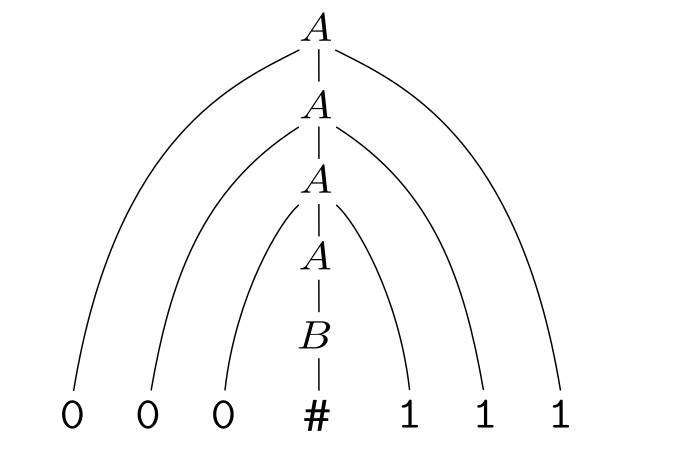
\includegraphics[scale=0.3]{figur/figur21.png}
	\end{center}
	\begin{itemize}
		\item Alle strenge der kan genereres fra \eqref{eq:cfgex} er dele af \textit{sproget af grammatikken}, som skrives $L(G_{1})$.
		\item \textbf{Ethvert sprog der kan genereres af en CFG er et kontekstfrit sprog}. (Definition, ikke sætning.)
	\end{itemize}
\end{frame}

\begin{frame}
	\frametitle{Formel Definition af Kontekstfri Grammatik}
	\begin{definition}[Kontekstfri Grammatik]
		En kontekstfri grammatik er en 4-tuple $(V, \Sigma, R, S)$, hvor
		\begin{enumerate}
			\item $V$ er en endelig mængde kaldet \textit{variabler}
			\item $\Sigma$ er en endelig mængde disjunkt fra $V$, kaldet \textit{terminaler}
			\item $R$ er en endelig mængde af \textit{regler}, hvor hver regel er en variabel (venstresiden) og en streng af variabler og terminaler (på højresiden)
			\item $S \in V$ er startvariablen
		\end{enumerate}
	\end{definition}
\end{frame}

\begin{frame}
	\frametitle{Kontekstfrie grammatikker, fortsat}

	\begin{itemize}
		\item Hvis $uAw$ kan blive til $uwv$, siger vi at $uAv$ \textit{giver} $uwv$, og skriver det $uAv \Rightarrow uwv$.
		\item Vi siger at $u$ \textit{udleder} (ikke afleder!) $v$ hvis der eksisterer en udledning $u \Rightarrow u_{1} \Rightarrow u_{2} \Rightarrow \cdots \Rightarrow u_{k} \Rightarrow v$.
		      \begin{itemize}
			      \item Vi skriver dette $u \overset{*}{\Rightarrow} v$ hvis $u = v$
		      \end{itemize}
		\item Sproget af en grammatik er dermed $\{w \in \Sigma^{*} \mid S \overset{*}{\Rightarrow}\}$
	\end{itemize}
\end{frame}

\begin{frame}[allowframebreaks]
	\frametitle{Tvetydighed}

	\begin{itemize}
		\item Hvis en grammatik kan generere den samme streng på mere end én forskellig måde, siger vi at strengen er afledt tvetydigt i den grammatik.
		\item Hvis en grammatik kan generere en streng tvetydigt, siger vi at selve grammatikken er \textit{tvetydig}.
	\end{itemize}

	\begin{equation}
		\langle \text{EXPR} \rangle \rightarrow \langle \text{EXPR} \rangle + \langle \text{EXPR} \rangle \mid \langle \text{EXPR} \rangle \times \langle \text{EXPR} \rangle \mid ( \langle \text{EXPR} \rangle ) \mid a
	\end{equation}

	\begin{itemize}
		\item Den ovenstående grammatik er tvetydig, da den generer strengen $a+a \times a$ tvetydigt.
		\item Vi kan se dette ved at lave to forskellige parsetræer:
	\end{itemize}

	\begin{center}
		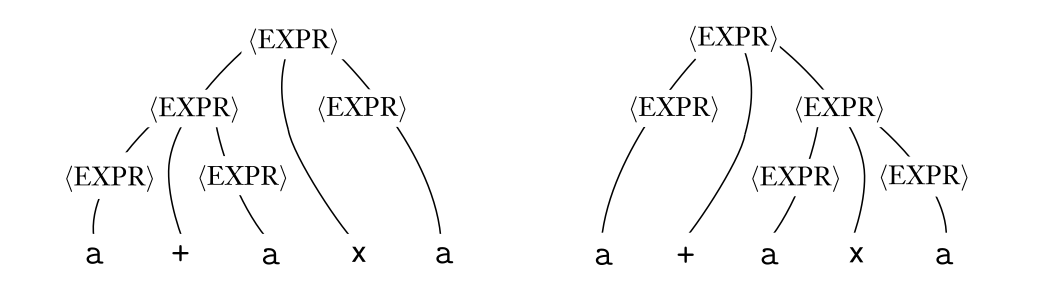
\includegraphics[scale=0.3]{figur/figur26.png}
	\end{center}
	\begin{itemize}
		\item Der eksisterer sproge der kun kan genereres af tvetydige grammatikker.
		\item Disse sprog siges at være \textit{i sig selv tvetydige}.
	\end{itemize}
\end{frame}

\begin{frame}[allowframebreaks]
	\frametitle{Chomsky Normal Form}

	\begin{itemize}
		\item (også kaldt, af Jørgen, Chomsky grammar).
		\item Chomsky Normal Form er en speciel \textit{form} til kontekstfrie grammatikker.
		\item Chomsky Normal Form sikrer nogle specifikke ting, der gør den brugbar til f.eks. algoritmer og beviser.
	\end{itemize}

	\begin{definition}[Chomsky Normal Form]
		En kontekstfri grammatik er i CNF hvis hver regel er af formen
		\begin{align*}
			A & \rightarrow BC \\
			A & \rightarrow a
		\end{align*}
		hvor $a$ er en vilkårlig terminal, og $A, B$ og $C$ er variabler, undtagen at $B$ og $C$ \textit{ikke} må være startvariablen. Vi tillader deruover også reglen $S \rightarrow \varepsilon$, hvor $S$ er startvariablen.
	\end{definition}

	\begin{theorem}
		Ethvert kontekstfrit sprog er genereret af en kontekstfri grammatik i CNF.
	\end{theorem}

	\begin{itemize}
		\item Vi kan konvertere en grammatik $G$ til CNF.
		\item Vi kan gøre dette ved at, trinvist, fjerne regler der ikke overholder betingelserne, og erstatter med regler der overholder.
		\item Først tilføjer vi en ny startvariabel.
		\item Så fjerner vi alle $\varepsilon$-regler af formen $A \rightarrow \varepsilon$.
		\item Vi eliminerer også alle \textit{unit regler} af formen $A\rightarrow B$.
		\item Til sidst konverterer vi de resterende regler til den rigtige form.
		\item \textbf{Bevis:}
	\end{itemize}
	\begin{enumerate}
		\item Først laver vi en ny startvariabel $S_{0}$, og tilføjer reglen $S_{0} \rightarrow S$, hvor $S$ var den tidligere variabel. Dermed sikrer vi at startvariablen ikke er på højresiden.
		\item Derefter tager vi os af epsilon-reglerne. Vi fjerner alle regler $A \rightarrow \varepsilon$ hvor $A$ ikke er starvariablen. \\ Derefter, for hver $A$ på højresiden af en regel, tilføjer vi en ny regel hvor vi fjerner $A$. Altså hvis $R \rightarrow uAv$ er en regel, tilføjer vi reglen $R \rightarrow uv$. Vi gørt dette for hvert tilfælde af $A$, så $R \rightarrow uavAw$ giver us tre regler: $R \rightarrow uvAw, R \rightarrow uAvw$ og $R \rightarrow uvw$. \\ Hvis reglen $R \rightarrow A$ eksisterer, erstatter vi denne med $R\rightarrow \varepsilon$, undtagen hvis $R \rightarrow \varepsilon$ er en regel vi allerede har fjernet. \\ Vi gentager dette indtil vi har fjernet alle epsilon-regler.
		\item Derefter fjerner vi alle \textit{unit regler}, altså for hvert $A \rightarrow B$ fjerner vi denne, og for alle $B \rightarrow u$, tilføjer vi $A \rightarrow u$, undtagen hvis dette er en regel vi allerede har fjernet, hvor $u$ er en streng af terminale og variabler. Vi gentager indtil alle unit regler er fjernet.
		\item Sidst konverterer vi alle tilbagestående regler til den rigtige form. For hvert $A \rightarrow u_{1}u_{2} \ldots u_{k}, k \ge 3$ fjerner vi denne regel, og tilføjer reglerne $A \rightarrow u_{1}A_{1}$, $A_{1} \rightarrow u_{2}A_{2}$, $A_{2} \rightarrow u_{3}A_{3}, \ldots A_{k-2} \rightarrow u_{k-1}u_{k}$
	\end{enumerate}
\end{frame}


\frametitle{CFG Konverting Eksempel}
Vi kigger på eksempel 2.10 pp. 110 i bogen for bedring af forståelse.
\end{frame}

\subsection{Pushdown Automater}%
\label{subsec:pda}


\begin{frame}[allowframebreaks]
	\frametitle{Pushdown Automater}
	\begin{itemize}
		\item Pushdown Automater (PDA) er ligesom NFA'er, men med en tilsluttet stak.
		\item Denne stak tillader pushdown automater at genkende flere sprog end en normal endelig automat, da den giver en uendelig hukommelse.
		\item Overførselsfunktionen for en PDA tillader dermed også \textit{pushing} og \textit{popping} af stakken.
		\item Stakken fungerer LIFO, og har dermed begrænset hukommelse.
		\item Sproget $\{0^{n}1^{n} \mid n \ge 0\}$ er et eksempel på et sprog der kan genkendes når vi nu har en stak:
		      \begin{itemize}
			      \item For hvert \texttt{0} der er læst, push det til stakken.
			      \item Når et \texttt{1} læses, pop for hvert 1 der er læst.
			      \item Hvis stakken er tom når der ikke er flere \texttt{1}'ere, så \textit{accepter}, ellers \textit{afvis}.
		      \end{itemize}

		\item En PDA er nondeterministisk, og er \textit{ikke} ækvivalent i sin deskriptive kraft til deterministiske automater med en stak. Disse genkender færre sprog.
	\end{itemize}
\end{frame}

\begin{frame}[allowframebreaks]
	\frametitle{Formel Definition af en Pushdown Automat}
	\begin{itemize}
		\item Det er ikke nødvendigt at bruge samme alfabet til input og til stak, dermed lader vi inputalfabetet være $\Sigma$ og stakalfabetet være $\Gamma$.
		\item Dermed er overførselsfunktionens domæne $Q \times \Sigma_{\varepsilon} \times \Gamma_{\varepsilon}$.
		\item Værdimængden fungerer som typisk ved nondeterminisme, men inklusiv stakken, da den også kan ændres. Dermed bliver værdimængden $\mathcal{P}(Q \times \Gamma_{\varepsilon})$.
	\end{itemize}

	\begin{definition}[Pushdown Automat]
		En \textit{pushdown automat} er en 6-tuple ($Q, \Sigma, \Gamma, \delta, q_{0}, F$), hvor $Q, \Sigma, \Gamma$ og $F$ alle er endelige mængder, og
		\begin{enumerate}
			\item $Q$ er mængden af tilstande
			\item $\Sigma$ er inputalfabetet
			\item $\Gamma$ er stakalfabetet
			\item $\delta : Q \times \Sigma_{\varepsilon} \times \Gamma_{\varepsilon} \longrightarrow \mathcal{P}(Q \times \Gamma_{\varepsilon})$ er overførselsfunktionen
			\item $q_{0} \in Q$ er starttilstanden
			\item $F \subseteq Q$ er mængden af accepttilstande
		\end{enumerate}
	\end{definition}

	\begin{itemize}
		\item Komputeringen i en pushdown automat fungerer som følge:
		\item Lad input $w$ være et input der accepteres hvis $w$ kan skrives $w = w_{1}, \ldots, w_{n}, $, hvor $\forall w_{i} : w_{i} \in \Sigma_{\varepsilon}$.
		\item En sekvens af tilstande $r_{0}, r_{1}, \ldots, r_{m} \in Q$ og strengene $s_{0}, s_{1}, \ldots, s_{m} \in \Gamma^{*}$ eksisterer som opfylder følgende tre betingelser:
		      \begin{enumerate}
			      \item $r_{0} = q_{0}$ og $s_{0} = \varepsilon$
			      \item $i = 0, \ldots, m-1 : (r_{i+1}, b) \in \delta(r_{i}, w_{i+1}, a)$, hvor $s_{i} = at$ og $s_{i+1} = bt$, hvor $a,b \in \Gamma_{\varepsilon}$ og $t \in \Gamma^{*}$. I.e., bevæger $M$ sig ifølge tilstanden, stakken og det næste inputsymbol.
			      \item $r_{m} \in F$. Denne betingelse siger at en accepttilstand forekommer i inputtets slutning.
		      \end{enumerate}
	\end{itemize}
\end{frame}

\begin{frame}[allowframebreaks]
	\frametitle{Eksempel 2.14}

	\begin{itemize}
		\item Vi vil nu beskrive en PDA der genkender $\{0^{n}1^{n} \mid n \ge 0\}$.
		\item Lad $M_{1} = (Q, \Sigma, \Gamma, \delta, q_{1}, F)$, hvor
		      \begin{enumerate}
			      \item[$Q = $] $\{q_{1}, q_{2}, q_{3}, q_{4}\}$
			      \item[$\Sigma = $] $\{0, 1\}$
			      \item[$\Gamma = $] $\{0, \mathdollar \}$
			      \item[$F = $] $\{q_{1}, q_{4}\}$
			      \item[$\delta = $]
			            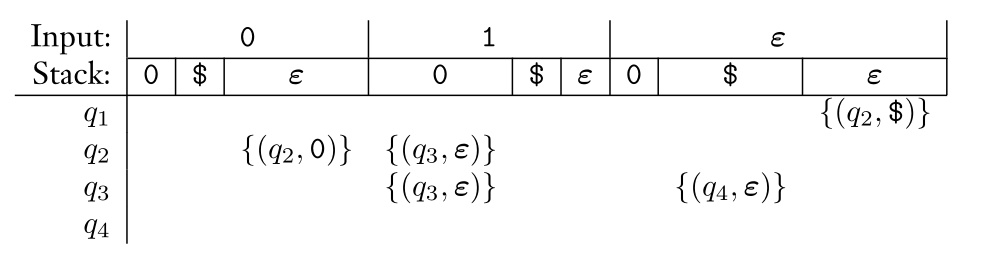
\includegraphics[scale=0.3]{figur/eksempel214.png}
		      \end{enumerate}

		\item Vi kan også lave en tilstandsdiagram. Bemærk her at $a,b \longrightarrow c$ betyder ``læs et $a$ fra input, erstat $b$ fra stakken med $c$'': \\
		      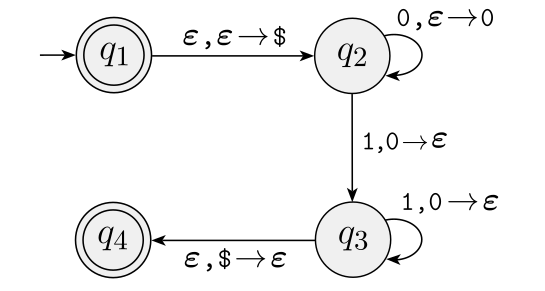
\includegraphics[scale=0.4]{figur/figur215.png}
	\end{itemize}
\end{frame}

\begin{frame}[allowframebreaks]
	\frametitle{Ækvivalens med Kontekstfrie Grammatikker}
	\begin{theorem}
		Et sprog er kontekstfrit hvis og kun hvis ($\iff$) en pushdown automat genkender det.
	\end{theorem}

	\begin{lemma}
		Hvis et sprog er kontekstfrit, så genkender en pushdown automat det.
	\end{lemma}

	\begin{itemize}
		\item Vi gør ligesom i bogen og kommer først med idéen, og derefter selve beviset:
		\item Vores mål er at vise at en CFG $G$ der genkender $A$ kan konverteres til en ækvivalent PDA $P$.
		\item PDA'en fungerer ved at acceptere input $w$ hvis $G$ genererer denne streng. Den finder ud af dette ved at finde ud af om der findes en afledning for $w$.
		\item Vi kalder en streng af variabler og terminaler der ikke er sluttet (afledt) og ikke er startstrengen for en \textit{mellemliggende streng} (intermediate string).
		\item Følgende er en uformel beskrivelse af PDA'en $P$:
		      \begin{enumerate}
			      \item Placer markeringssymbolet $\mathdollar$ og startvariablen på stakken
			      \item Gentag følgende skridt forevigt:
			            \begin{enumerate}
				            \item Hvis toppen af stakken er et variabelsymbol $A$, vælg nondeterministisk en af reglerne og erstat med højrehåndssiden.
				            \item Hvis toppen er et terminalsymbol, læs det næste symbol fra inputtet og sammenlign med $a$. Hvis de er lig hinanden, så gentag. Hvis ikke, så \textit{afvis} denne gren.
				            \item Hvis toppen af stakken er symbolet $\mathdollar$, gå til \textit{accepttilstanden}.
			            \end{enumerate}
		      \end{enumerate}

		\item Vi vil nu formalisere dette bevis.
		\item Lad $P = (Q, \Sigma, \Gamma, \delta, q_{start}, F)$ være en PDA.
		\item Vi laver en forsimplet notation til overførselsfunktionen:
		\item Lad $q$ og $r$ være tilstande i PDA'en, og lad $a \in \Sigma_{\varepsilon}, s \in \Gamma_{ \varepsilon}$.
		\item Vi vil gerne gå fra $q$ til $r$ når den læser $a$ og popper $s$.
		\item Derudover skal den pushe strengen $u = u_{1}, \ldots u_{l}$ til stakken på samme tid.
		\item Vi implmenterer denne handling ved at introducere nye tilstande $q_{1}, \ldots, q_{l-1}$, og lade overførselsfunktionen være som følger:
		      \begin{align*}
			       & \delta(q,a,s) \text{ indeholder } (q_{1}, u_{l}),              \\
			       & \delta(q_{1}, \varepsilon, \varepsilon) = \{(q_{2}, u_{l-1})\} \\
			       & \delta(q_{2}, \varepsilon, \varepsilon) = \{(q_{3}, u_{l-2})\} \\
			      \vdots                                                            \\
			       & \delta(q_{l-1}, \varepsilon, \varepsilon) = \{(r, u_{1})\}
		      \end{align*}

		\item Vi kan grafisk se implementering her:
		      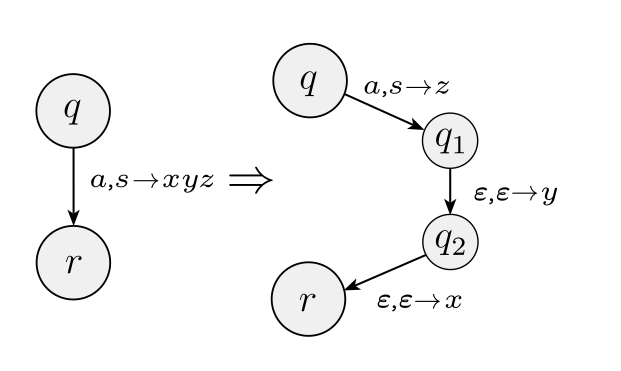
\includegraphics[scale=0.5]{figur/figur223.png}
		\item Tilstandene i $P$ er $Q = \{q_{start}, q_{gentag}, q_{accept}\} \cup E$ hvor $E$ er mængden af tilstandene vi skal bruge for at implementere \(\delta\). Ydermere $F = \{q_{accept}\}$.
		\item Vi definerer overførselsfunktionen som følger:
		      \begin{itemize}
			      \item Lad stakken starte med symbolerne $\mathdollar, S$. Det gør vi ved at bruge vores notation, $\delta(q_{start}, \varepsilon, \varepsilon) = \{(q_{loop}, S \mathdollar)\}$
			      \item Som det næste skal vi håndtere toppen af stakken. Til dette er der tre muligheder:
			            \begin{enumerate}
				            \item Toppen af stakken er en variabel\\ Lad $\delta(q_{loop}, \varepsilon, A) = \{(q_{loop}, w) \mid \text{ hvor } A \rightarrow w \text{ er en regel i }R\}$
				            \item Toppen af stakken er en terminal\\ Lad $\delta(q_{loop}, a, a) = \{(q_{loop}, \varepsilon)\}$
				            \item Toppen af stakken er tom (\textdollar) \\ Lad $\delta(q_{loop}, \varepsilon, \mathdollar) = \{(q_{accept}, \varepsilon)\}$
			            \end{enumerate}
		      \end{itemize}

		\item Vi kan se dette grafisk om følger:

		      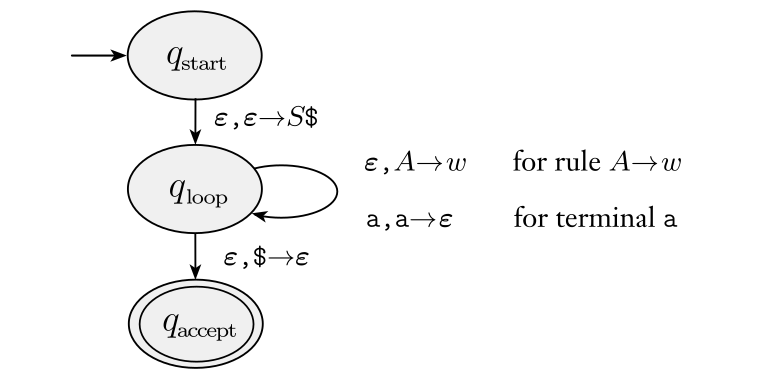
\includegraphics[scale=0.3]{figur/figur224.png}
	\end{itemize}
\end{frame}

\begin{frame}[allowframebreaks]
	\frametitle{Eksempel 2.25}

	\begin{itemize}
		\item Vi kigger hurtigt på et eksempel. Vi konstruerer en PDA fra CFG'en $G$:
	\end{itemize}
	\begin{align*}
		S & \rightarrow aTb \mid b          \\
		T & \rightarrow Ta \mid \varepsilon
	\end{align*}

	\begin{itemize}
		\item Overførselsfunktionen (samt hele tilstandsdaigrammet) kan ses i følgende diagram:
	\end{itemize}
	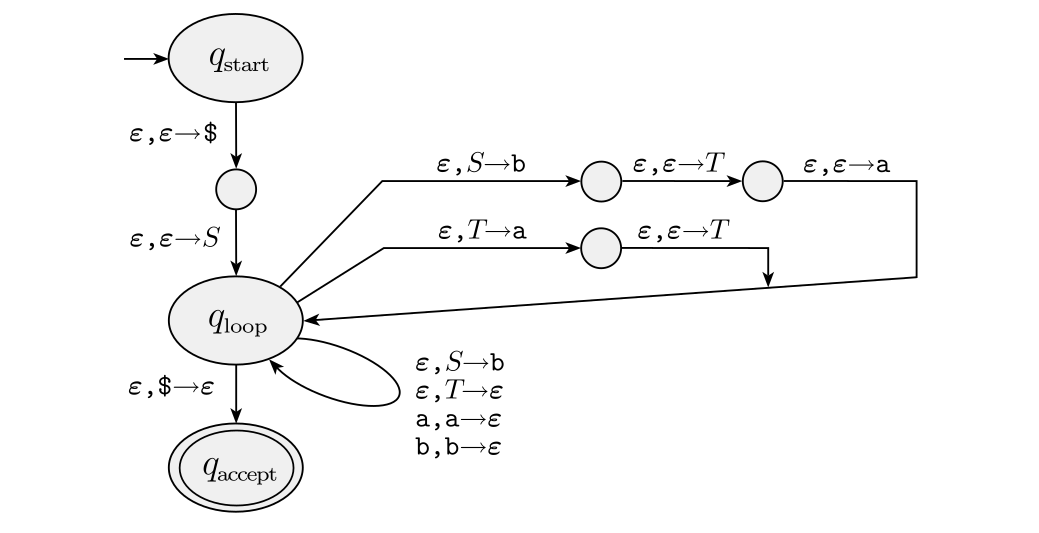
\includegraphics[scale=0.3]{figur/figur226.png}
\end{frame}

\begin{frame}[allowframebreaks]
	\frametitle{Ækvivalens Med Kontekstfrie Grammatikker 2}
	\begin{itemize}
		\item Vi vil nu bevise den anden retning.
	\end{itemize}

	\begin{lemma}
		Hvis en PDA genkender et sprog, så er det kontekst-frit.
	\end{lemma}

	\begin{itemize}
		\item Givet en PDA $P$, og en CFG $G$:
		\item For hvert par af states, $p$ og $q$ i $P$, vil vi have en variabel i grammatikken $A_{pq}$.
		\item Formålet med denne variabel er at den skal kunne generere alle strenge som kan tage $P$ fra $p$ med en tom stak til $q$ med en tom stak. Dette vil også betyde at stakken ikke ændrer sig overhovedet.
		\item Vi starter med at ændre lidt i $P$:
		      \begin{enumerate}
			      \item Den har én accept state $q_{accept}$
			      \item Den tømmer sin stak før den accepterer
			      \item Hver overførsel pusher enten et symbol til stakken eller popper et symbol fra stakken. Men ingen på samme tid.
		      \end{enumerate}
		\item Det er nemt at ændre i $P$ for at få den ønskede funktionalitet.
		\item For den 3. ændrer vi hver overførsel som både popper og pusher med to overførsler.
		\item Hver overførsel der hverken pusher eller popper, ændrer vi til to, hhv. en der først pusher og en der så popper.
		\item Vi ved at ved at gå fra en state $p$ til $q$ i PDA'en, givet en streng $x$, skal der \textit{pushes} før der kan \textit{poppes}. Vi ved dette præcis fordi vi antager at stakken er tom, eller at den i det mindste ikke ændrer på stakken. Dermed på der ikke poppes noget.
		\item Der er to muligheder, når $P$ kører på $x$:
		      \begin{enumerate}
			      \item Symbolet poppet i slutningen er symbolet pushet i starten.
			      \item Symbolet poppet i slutningen er \textit{ikke} symbolet pushet i starten.
		      \end{enumerate}

		\item Hvis (1) betyder det at stakken kun har været tom 2 gange: Før første push, og efter sidste pop.
		\item Hvis (2) må det første symbol blive poppet på et eller andet tidspunkt før $x$ er færdigkomputeret.
		\item Ved (1) kan vi simulere dette med reglen $A_{pq} \rightarrow aA_{rs}b$ hvor:
		      \begin{itemize}
			      \item $a$ er inputtet læst ved første overførsel
			      \item $b$ er inputtet læst ved sidste overførsel
			      \item $r$ er tilstanden efterfølgende $p$, og $s$ er tilstanden før $q$
		      \end{itemize}
		\item Ved (2) kan vi simulere den med reglen $A_{pq} \rightarrow A_{pr}A_{rq}$, hvor $r$ er tilstanden når stakken bliver tom.

		\item Visuelt forklaring for (1): 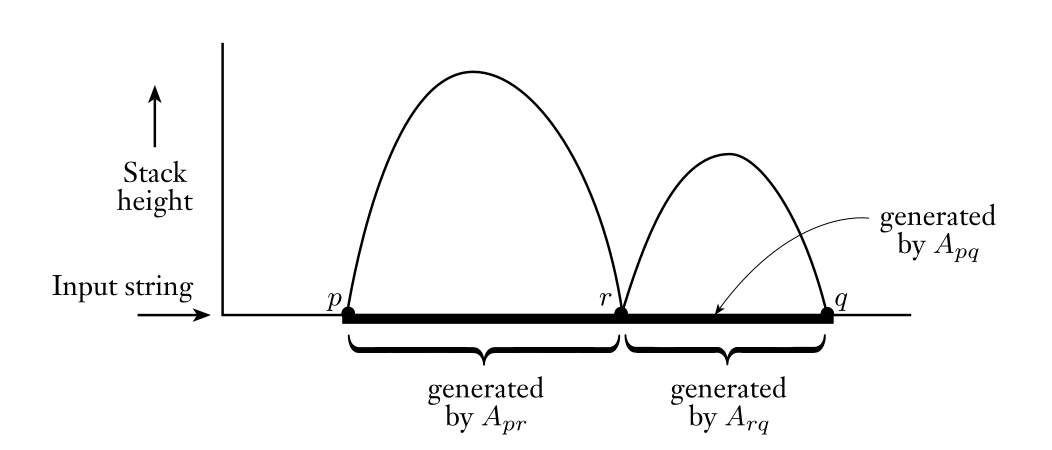
\includegraphics[scale=0.3]{figur/figur228.png}
		\item Visuelt forklaring for (2): 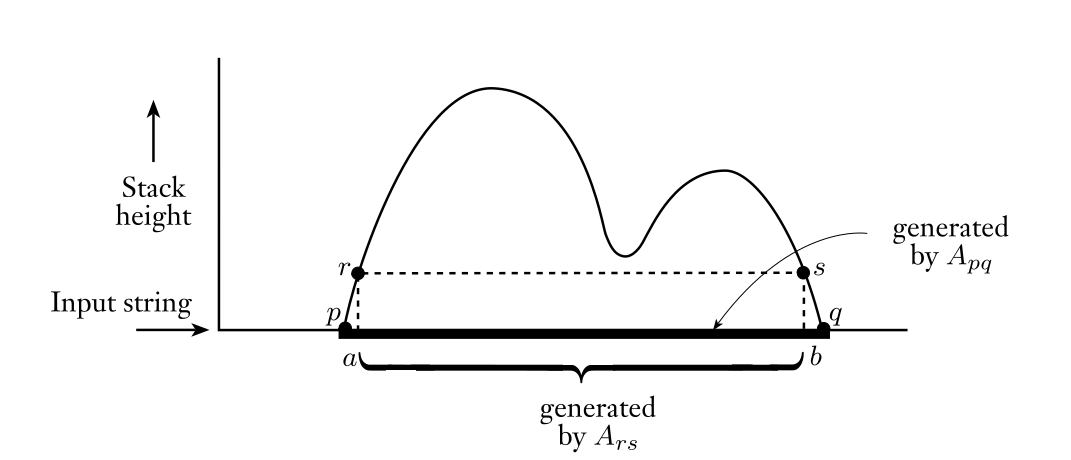
\includegraphics[scale=0.3]{figur/figur229.png}

		\item Nu til det formelle bevis (piv :( )
		\item Lad $P = (Q, \Sigma, \Gamma, \delta, q_{0}, \{q_{accept}\})$ og konstruer $G$.
		\item Variablerne af $G$ er $\{A_{pq} \mid p,q \in Q\}$
		\item Startvariablen er $A_{q_{0}, q_{accept}}$
		\item Vi beskriver $G$'s regler i tre dele:
		      \begin{enumerate}
			      \item For hvert $p,q,r,s \in Q, u \in \Gamma$ og $a,b \in \Sigma_{\varepsilon}$, hvis $\delta(p,a,\varepsilon)$ indeholder $(r,u)$ og $\delta(s,b,u)$ indeholder $(q, \varepsilon)$, put reglen $A_{pq} \rightarrow aA_{rs}b$ i $G$.
			      \item For hvert $p,q,r \in Q$, put reglen $A_{pq} \rightarrow A_{pr}A_{rq}$ i $G$
			      \item For hvert $p \in Q$, put reglen $A_{pp} \rightarrow \varepsilon$ i $G$
		      \end{enumerate}

		\item \textbf{Påstand}:
		      Hvis $A_{pq}$ genererer $x$, så kan $x$ bringe $P$ fra $p$ på en tom stak til $q$ med en tom stak.
		\item Vi beviser ved induktion.
		\item \textit{Basis}: Afledningen har ét skridt. Dette er trivielt bevist ved vores regel $A_{pp} \rightarrow \varepsilon$.
		\item \textit{Induktionsskridt}: Vi antager at det er sandt for afledninger af længde højest $k$, hvor $k \ge 1$, og beviser at det også gælder afledninger af længde $k+1$:
		\item Antag at $A_{pq} \overset{*}{\Rightarrow} x$ på $k+1$ skridt.
		\item Det første skridt i den afledning er enten $A_{pq} \Rightarrow aA_{rs}b$ eller $A_{pq} \Rightarrow A_{pr}A_{rq}$. Vi håndterer de to tilfælde seperat.
		\item I første tilfælde, lad os tænke på strengen i henhold til $y$, således at vi kan opdele $x$ til at være $x = ayb$, hvor $a$ og $b$ kender vi allerede.
		\item Fordi $A_{rs} \overset{*}{\Rightarrow} y$ med $k$ skridt, siger induktionshypotesen at $P$ kan gå fra $r$ på en tom stak til $s$ på en tom stak.
		\item Fordi $A_{pq} \rightarrow aA_{rs}b$ er en regel af $G$, indeholder $\delta(p,a,\varepsilon)$ $(r,u)$ og $\delta(s,b,u)$ indeholder $(q, \varepsilon)$, for et staksymbol $u$.
		\item Dermed, hvis $P$ starter på $p$ med en tom stak, efter at have læst $a$ kan den gå til tilstand $r$ og pushe $u$ til stakken.
		\item Så kan den læse strengen $y$ og bringe den til $s$ og lade $u$ være på stakken.
		\item Dermed, efter at have læst $b$ kan den gå til tilstand $q$ og poppe $u$ af stakken.
		\item Så $x$ kan gå fra $p$ på en tom stak til $q$ på en tom stak.
		\item I det andet tilfælde, antag at portionerne $y$ og $z$ af $x$  som $A_{pr}$ og $A_{rq}$ hhv. genererer, så $x = yz$.
		\item Fordi $A_{pr} \overset{*}{\Rightarrow} y$ på højest $k$ skridt og $A_{rq} \overset{*}{\Rightarrow} z$ på højest $k$ skridt, siger induktionshypotesen at $y$ kan bringe $P$ fra $p$ til $r$ og $z$ kan bringe $P$ fra $r$ til $q$ med en tom stak fra begyndelsen til slutningen. Dermed kan $x$ bringe den fra $p$ på en tom stak til $q$ med en tom stak.
		\item \textbf{Påstand}: Hvis $x$ kan bringe $P$ fra $p$ på en tom stak til $q$ på en tom stak, genererer $A_{pq}$ strengen $x$.
		\item Vi beviser igen ved induktion :)
		\item \textit{Basisskridt}. Komputeringen har $0$ skridt. Hvis komputeringen har 0 skridt starter og ender den på samme tilstand, e.g. $p$. Vi skal altså vise at $A_{pp} \overset{*}{\Rightarrow} x$. På 0 skirdt kan $P$ ikke læse nogen karakterer, så $x = \varepsilon$. Ved konstruktion, har $G$ reglen $A_{pp} \rightarrow \varepsilon$.
		\item \textit{Induktionsskridt}: Antag sand for komputationer af længde højest $k$, hvor $k \ge 0$, og bevis for $k+1$:
		\item Antag at $P$ har en komputering hvor $x$ bringer $p$ til $q$ på en tom stak i $k+1$ skridt.
		\item Så er stakken enten kun tom i begyndelsen og slutningen, eller den bliver tom på en eller flere tidspunkter mellem disse to.
		\item I første tilfælde (kun tom to gange) er symbolet der puishes i første overførsel det samme som symbolet der poppes i sidste overførsel.
		\item Vi kalder dette symbol $u$.
		\item Lad $a$ være inputtet læst i første overførsel og $b$ inputtet i sidste overførsel.
		\item Lad $r$ være tilstanden efter første overførsel, og $s$ tilstanden før sidste.
		\item Med det vil $\delta(p,a,\varepsilon)$ indeholde $(r,u)$ og $\delta(s,b,u)$ vil indeholder $(q,\varepsilon)$.
		\item Dermed er reglen $A_{pq} \rightarrow aA_{rs}b$ i $G$
		\item Lad $y$ være portionen af $x$ uden $a$ eller $b$, så $x = ayb$.
		\item Input $y$ kan bringe $P$ fra $r$ til $s$ på en tom stak uden at røre symbolet $u$ som er på styakken.
		\item Vi har fjernet første og sidste skridt af de $k+1$ skridt i den originale komputering af $x$, så komputeringen på $y$ har $(k+1)-2 = k-1$ skridt.
		\item Dermed siger induktionshypotesen at $A_{rs} \overset{*}{\Rightarrow} y$. Dermed $A_{pq} \overset{*}{\Rightarrow} x$.
		\item I andet tilfælde (3 eller flere gange der er en tom stak):
		\item Lad $r$ være en tilstand hvor stakken bliver tom andet end i begyndelsen eller slutningen af komputeringen på $x$.
		\item Så indeholder portionen af komputeringen fra $p$ til $r$ og fra $r$ til $q$ højest $k$ skridt.
		\item Hvis $y$ er inputet læst i første portion og $z$ i anden, så siger induktionshypotesen at $A_{pr} \overset{*}{\Rightarrow} y$ og $A_{rq} \overset{*}{\Rightarrow} z$. Fordi reglen $A_{pq} \rightarrow A_{pr}A_{rq}$ er i $G$, $A_{pq} \overset{*}{\Rightarrow} x$.
	\end{itemize}
\end{frame}

\begin{frame}[allowframebreaks]
	\frametitle{Jørgens Noter}
	\begin{itemize}
		\item En pushdown-automat (PDA) er en ikke-deterministisk endelig automat med en stak, hvilket gør PDA'er mere kraftfulde end DFA'er og NFA'er.
		\item Hvis en PDA skal være deterministisk, mister den evnen til at genkende visse sprog. Dette sker ikke for endelige automater.
		\item Et vigtigt faktum uden bevis (se papiret under noter på hjemmesiden) er, at hvert kontekstfrit sprog over et ét-symbols alfabet også er regulært. Du skal kunne bruge dette faktum, men ikke bevise det.
		\item Der findes sprog, der ikke er kontekstfrie, og pumpesætningen kan bruges til at bevise dette ved modstrid. Et eksempel er $\{a^n b^n c^n \mid n \geq 0\}$.
		\item Hvert regulært sprog er kontekstfrit.
		\item Klassen af kontekstfrie sprog er ikke lukket under fællesmængde. Der findes kontekstfrie sprog $L_1$ og $L_2$, hvor $L_1 \cap L_2$ ikke er kontekstfrit. For eksempel, hvis $L_1 = \{a^i b^j c^k \mid i, j, k \geq 0 \text{ og } i = j\}$ og $L_2 = \{a^i b^j c^k \mid i, j, k \geq 0 \text{ og } j = k\}$, så er både $L_1$ og $L_2$ kontekstfrie, men $L_1 \cap L_2 = \{a^n b^n c^n \mid n \geq 0\}$, hvilket ikke er kontekstfrit.
		\item PDA'er er ækvivalente med kontekstfrie grammatikker. For enhver PDA $A$ kan man konstruere en grammatik $G$ sådan at $L(A) = L(G)$, og omvendt.
		\item Klassen af kontekstfrie sprog er lukket under foreningsmængde, sammenkædning og stjerne, men ikke under fællesmængde og komplement. Dette betyder ikke, at komplementet af et kontekstfrit sprog aldrig er kontekstfrit. For eksempel er både $\Sigma^*$ og dets komplement, den tomme mængde, kontekstfrie (også regulære). Ligeledes er $L = \{a^n b^n \mid n \geq 0\}$ og dets komplement kontekstfrie (men ikke regulære).
		\item Fællesmængde af et kontekstfrit sprog $L_1$ med et regulært sprog $L_2$ er kontekstfrit. Hvis vi har en PDA $M_1$ for $L_1$ over $\Sigma$ og en DFA $M_2$ for $L_2$, kan vi lave en PDA $M$ som simulerer $M_1$ og $M_2$ parallelt. Den nye PDA $M$ har par af tilstande $(q, p)$, hvor $q$ er den aktuelle tilstand af $M_1$ og $p$ den aktuelle tilstand af $M_2$. Når $M$ læser et symbol $a \in \Sigma$, opdaterer den både $M_1$'s tilstand og stak samt $M_2$'s tilstand. $M$ accepterer en streng $w$ hvis og kun hvis både $M_1$ accepterer $w$ (med tom stak) og $M_2$ accepterer $w$. Derfor er $L_1 \cap L_2$ kontekstfrit, da det accepteres af en PDA.
	\end{itemize}
\end{frame}






%%% mode: latex
%%% TeX-engine: xetex
%%% TeX-command-extra-options: "-shell-escape"
%%% TeX-master: "main"
%%% End:

\chapter{Turingmaskiner}

\section{Turingmaskiner}%
\label{sec:label}

En Turingmaskine minder om en endelig automat, men med et uendeligt og ubegrænset bånd (fremfor et uendeligt men begrænset bånd som i en PDA). I overføringsfunktionen bestemmes om hovedet på båndet går til venstre eller højre, og hvad den skriver, hvis noget, givet hvad der allerede står på båndet. En Turingmaskine har 3 specielle tilstande:
\begin{itemize}
	\item $q_{0}$: Den initielle tilstand
	\item $q_{acc}$: Den accepterence tilstand
	\item $q_{rej}$ Den afvisende tilstand
\end{itemize}

Både den accepterende og den afvisende tilstand træder i kraft så snart de nåes, altså stopper en Turingmaskine hvis en af disse nåes.

Der findes mange forskellige varianter af Turingmaskiner (som vi kommer ind på senere), men den \textit{konventionelle} Turingmaskine har et uendeligt bånd til højre, men har en start til venstre.

Følgende er den formelle definition af en Turingmaskine:

\begin{definition}[Formel Definition af en Turingmaskine]
	\label{def:formalturing}
	En \textbf{Turingmaskine} er en 7-tuple $(Q, \Sigma, \Gamma, \delta, q_{0}, q_{\text{accept}}, q_{\text{reject}})$, hvor $Q, \Sigma, \Gamma$ alle er endelige sæt, og
	\begin{enumerate}
		\item $Q$ er sættet af states.
		\item $\Sigma$ er inputalfabetet ikke indeholdende det blanke symbol, $\sqcup$.
		\item $\Gamma$ er båndalfabetet, hvor $\sqcup \in \Gamma$ og $\Sigma \subseteq \Gamma$.
		\item $\delta, Q \times \Gamma \longrightarrow Q \times \Gamma \times \{L, R\}$ er transitionsfunktionen.
		\item $q_{0} \in Q$ er startstaten.
		\item $q_{\text{accept}} \in Q$ er accept staten.
		\item $q_{\text{reject}} \in Q$ er afvis staten, hvor $q_{\text{accept}} \neq q_{\text{reject}}$.
	\end{enumerate}
\end{definition}

\subsection{Konfigurationer}%
\label{subsec:label}


En konfiguration er en indikation på hvor på båndet en Turingmaskine befinder sig, samt i hvilken tilstand. ``$uqv$'', $q \in Q, u, v \in \Gamma^{*}$ betyder at båndhovedet er over ``$v$'', og at vi er i tilstanden $q$.

Vi siger at en konfiguration $C_{1}$ \textit{giver} $C_{2}$ hvis $M$ kan gå fra $C_{1}$ til $C_{2}$ i ét skridt.

For eksempel $uaq_{i}bv \rightarrow uq_{j}acv$ (hvor \(\rightarrow\) betyder ``giver''), er det samme som $\delta(q_{i},b) = (q_{j}, c, L)$

Hvis hovedet forsøger at gå til venstre, når den allerede er på den venstremest position, vil den forblive der, og altså ikke flytte sig. Den kan sevlfølgelig stadig ændre på båndindholdet osv. Der er nogle der mener at en Turingmaskine der vil gå til venstre når den allerede er helt til venstre skal afvises, men sådan ser vi ikke på det. Altså $q_{i}bv \rightarrow q_{j}cv$ hvis $\delta(q_{i},b) = (q_{j}, c, L)$

Der er nogle specielle konfigurationer:

\begin{itemize}
	\item Startkonfigurationen $q_{0}w$ hvor $w$ er input
	\item Acceptkonfigurationen $uq_{acc}v$
	\item Afvisningskonfigurationen $u'q_{rej}v'$
\end{itemize}

Vi kan derfor definere alle sprog der accepteres af en Turingmaskine således:
\begin{equation}
	L(m) = \{w \mid q_{0}w \stackrel{*}{\longrightarrow} uq_{acc}v \text{ for en }u,v \in \Gamma^{*}\}
\end{equation}

$q_{0}w = c_{0} \rightarrow c_{1} \rightarrow c_{2} \rightarrow \cdots \rightarrow c_{n} = uq_{acc}v$

\begin{definition}
	$L$ er \textit{Turing-genkendeligt} (også kaldt rekursivt enumerabelt) $\iff$ $L = L(m)$ for en Turingmaskine $m$.
\end{definition}

Der er tre muligheder når en Turingmaskine $m$ starter på en streng $w$:
\begin{itemize}
	\item $m$ accepterer $w$: $q_{0}w \rightarrow uq_{acc}v$
	\item $m$ afviser $w$: $q_{0}w \rightarrow u'q_{rej}v'$
	\item $m$ kører for evigt
\end{itemize}

\begin{definition}[Afgører]
	En Turingmaskine $m$ er en \textit{afgører} hvis $m$ altid stopper.
\end{definition}

\begin{definition}
	$L$ er \textit{afgørligt} $\iff$ $L = L(m)$ for en afgører $m$.
\end{definition}

\section{Varianter af Turingmaskiner}%
\label{sec:label}

Som tidligere skrevet er der flere varianter af Turingmaskiner. Vi vil kigge på dem her, og gennemgå konvertering fra denne variant til vores enkeltbånds deterministiske Turingmaskine, som er den vi kender nu.

\subsection{Flere bånd}%
\label{subsec:label}

En variant af en Turingmaskine er en der har mere end ét bånd. Det kan være så mange bånd, som man ønsker, \textit{men} det kan ikke ændres i køretiden.

Overføringsfunktionen for en sådan Turingmaskine er lidt sjov: $\delta(q, a_{1}, a_{2}, \ldots, a_{k}) = (p, b_{1}, b_{2}, \ldots, b_{k}, \delta_{1}, \delta_{2}, \ldots, \delta_{k})$. Her går vi fra tilstand $q$ til $p$ og erstatter $a_{i}$ med $b_{i}$ og flytter hovedet ifølge $\delta_{i}$, hvor \(\delta \in \{L, R, S\}\).

En flerbånds Turingmaskine kan lave nogle ting hurtigere end en ``normal'' Turingmaskine. For eksempel kan den kopiere en streng i $O(|w|)$ tid ved brug af 2 bånd, hvor en normal ville bruge $O(|w|^{2})$ tid.

\subsection{2-vejs uendeligt bånd}%
\label{subsec:label}

Dette er en Turingmaskine hvor både venstre og højresiden er uendelig, og ikke kun højresiden.

\subsection{Nondeterministisk Turingmaskine}%
\label{subsec:label}

En nondeterministisk Turingmaskine, kontrær til en deterministisk Turingmaskine, kan gætte fra en tilstand $q$ på et symbol $a \in \Sigma$, hvor der kan være op til $B = |Q| \cdot |\Gamma| \cdot 3$ forskellige overføringer.

\subsection{Et bånd med flere hoveder}%
\label{subsec:label}

Denne variant af en Turingmaskine har mere end blot et enkelt hoved.

\subsection{To-dimensionelt Bånd}%
\label{subsec:label}

Det er også muligt at have en Turingmaskien hvis bånd nærmest er matriks-agtigt, som går uendeligt op og tilhøjre.

Bemærk at alle disse varianter kan konverteres til en deterministk Turingmaskine, dog med forskellige køretider (eksponentiel, i tilfældet af en NDTM).

\subsection{Konvertering af Flerbånds til Enkeltbånds}%
\label{subsec:label}

Når vi konverterer fra flere bånd til et enkelt bånd skal dette enkelte bånd kunne gøre atld et som flere bånd kunne, dog ikke (nødvendigvis) ligeså hurtigt. Vi indikerer på båndet skiftet mellem to bånd ved \#. Så eksempelvis kan \textit{\#aabb\#bbaa\#hhii} være 3 bånd med indholdet på aabb første bånd, bbaa på andet bånd og hhii på tredje bånd. Hvis et bånd vil videre til højre, så bruger vi blot rightshift. Vi simulerer hovederne ved at have et specielt symbol korresponderende til hvert symbol i maskinen. Jørgen bruger f.eks. $\stackrel{\circ}{a}$ til $a$.

Vi vil dog gerne se præcis hvordan vi implementerer den her simulering, hvor vi går fra $k$ bånd til ét.

Antag at $M$ er en $k$-bånds Turingmaskine. For hver tilstand $q_{i}$ af $M$ har vi følgende tilstande:
\begin{itemize}
	\item $q^{i}_{(\alpha_{1}, \alpha_{2}, \ldots, \alpha_{k})}$ hvor $a_{i} \in \Gamma \cup \{-\}$
	      \begin{itemize}
		      \item Her betyder $\{-\}$ at vi endnu ikke ved, hvad der skal stå der.
	      \end{itemize}
	\item $p^{i}_{(\delta_{1}, \delta_{2}, \ldots, \delta_{k}, b_{1}, b_{2}, \ldots, b_{k}, \gamma_{1}, \gamma_{2}, \ldots, \gamma_{k})}$ hvor $\delta_{i} \in \Gamma \cup \{-\}, b_{i} \in \Gamma, \gamma_{i} \in \{R, L, S\}$
\end{itemize}

Når vi er i tilstand $q^{i}_{(\beta_{1}, \beta_{2}, \ldots, \beta_{r}, -, -, \ldots, -)}$ har vi samlet symbolerne under hovederne i de første $r$ tilstande.

Når vi er i tilstand $p^{i}_{(b_{1}, \ldots, b_{q}, -, \ldots, -, b_{1}, \ldots, b_{k}, \gamma_{1}, \gamma_{2}, \ldots, \gamma_{k})}$ har vi ændfret på båndcellerne under de første $q$ hoveder og flyttet det $i$'e hoved ( hvor $i \le q$ ) ifølge $\gamma_{i}$ (og muligvis rightshiftet en del af båndet).

Bemærk at dette er \textit{utroligt} mange tilstande. For $q^{i}$ i sig selv er der $(\Gamma+1)^{k}$ muligheder. Ved $p^{i}$ er der $3^{k} \cdot \Gamma^{k} + (\gamma+1)^{k}$ muligheder. \textbf{Men} det er polynomielt!

Vi vil nu gå ind i hvordan man implementerer ét skridt \(\delta(q_{i}, a_{1}, a_{2}, \ldots, a_{k}) = (q_{j}, b_{1}, b_{2}, \ldots, b_{k}, \gamma_{1}, \gamma_{2}, \ldots, \gamma_{k})\):
\begin{enumerate}
	\item $M'$ starter i tilstanden $q^{i}_{(-,-,\ldots, -)}$ på den venstremest del af båndet.
	\item I tilstanden $q^{i}_{(a_{1}, \ldots, a_{r}, -,-, \ldots, -)}$ hvor $r < k$ bevæger $m'$ sit hoved fremad til at kopiere indeholdet under $M'$s $(r+1)$'e hoved.
	\item Når vi når til tilstanden $q^{i}_{(a_{1}, a_{2}, \ldots, a_{k})}, a_{i} \in \Gamma$ har vi samlet alle karaktererne under $M$'s hoveder og overfører til staten $p^{j}(-,\ldots,-,b_{1},\ldots, b_{k}, \gamma_{1}, \ldots, \gamma_{k})$ som afgænger af overføringsfunktionen ($p^{j}$ fordi overføringsfunktionen vil have os til $q_{j}$, hvor $p$ = predecessor, en der kommer før).
	\item I tilstanden $p^{j}_{(b_{1}, \ldots, b_{s}, -, \ldots, -, b_{1}, b_{2}, \ldots, b_{k}, \gamma_{1}, \gamma_{2}, \ldots, \gamma_{k})}$ hvor $s < k$, sker følgende:
	      \begin{itemize}
		      \item Flyt til positionen af det $(s+1)$'e hoved.
		      \item Erstat $a_{s+1}$ med $b_{s+1}$ ifølge overføringsfunktionen, og flyt det virtuelle hoved i forhold til \(\gamma_{s+1}\).
		      \item  Hvis $s+1 < k$ gå til tilstand $p^{j}_{(b_{1}, \ldots, b_{s+1}, - , \ldots, - , b_{1}, b_{2}, \ldots, b_{k}, \gamma_{1}, \ldots, \gamma_{k})}$ og start forfra. Ellers bevæg hovedet til den venstremest position og tå til tilstanden $q^{j}_{(-, \ldots, -)}$ da vi nu (endelig) er kommet til tilstanden $q_{j}$.
	      \end{itemize}
\end{enumerate}

\subsubsection{Køretid for Simuleringen}

Antag at $M$ tager $t$ skridt på input $w$, hvor $|w| = n$. Så kan inputtet højest indholde $ n  + t$ symboler udover det tomme symbol, og alle andre bånd har højest $t$ symboler udover det tomme symbol, da de starter med at være tomme.

Vi kigger på to muligheder, først at det ikke har været nødvendigt at lave nogen rightshifts, og derefter hvor det har været. At simulere et skridt hvor ingen rightshift har været nødvendigt tager $O(\Sigma \text{ længden af båndet}) = O(n+kt)$, hvor $n$ er længden af inputtet $w$ og $kt$ er skridt taget per bånd, $t$ ganget med antallet af bånd $k$.

Det er dog meget usandsynligt at der \textit{ikke} bliver lavet mange rightshifts. Hvis vi rightshifter hver eneste gang er der $O((k-1)t + (k-2)t + \cdots + t) = O(k^{2}t)$.

Det samlede arbejde for at simulere ét skridt er $O(n+kt) + O(k^{2}t) = O(n+k^{2}t)$. Det smalede arbejde for at simulere $t$ skridt er så $O(n \cdot t + k^{2}t^{2})$.

\subsection{Konverting af Nondeterministisk til Deterministisk}%
\label{subsec:label}

En nondeterministisk endelig automat har overføringsfunktionen $Q \times \Gamma \rightarrow \mathcal{P}(Q \times \Gamma \times \times \{L,R,S\})$. Dette er utroligt mange muligheder, \textbf{men det er ikke uendelige}! Der er $B$ muligheder, hvor $B \le |Q| \cdot |\Gamma| \cdot 3$. Vi kan se på komputeringen af en nondeterministisk Turingmaskine $M$ på  en streng $w$ som et træ, hvor hver knude har \textbf{højest} $B$ børn. Hver vej i dette træ korresponderer derfor til et specifikt valg for hver af tilstandene.


\begin{definition}
	Den nondeterministiske Turingmaskine $M$ \textit{genkender} $L$ hvis der er en komputering for $M$ på $w$ som leder til en accepttilstand.
\end{definition}
Altså behøver alle grene ikke føre til en accepttilstand.

\begin{definition}
	En nondeterministisk Turingmaskine $M$ \textit{afgører} $L$ hvis $\forall w \in \Sigma^{*}$:
	\begin{enumerate}
		\item \(\exists k = k(M, w)\) hvor $M$ aldrig tager mere end $k$ skridt på $w$.
		\item $w \in L \iff M$ har mindst en accepterende udregning på $w$.
	\end{enumerate}
\end{definition}

Altså er forskellen på en afgører og en genkendende nondeterministisk Turingmaskine bare at en afgører har en ``grænse'' på hvor lang hver vej er, hvor en genkendende ikke har, der behøver bare at være en accepterende tilstand.

\begin{theorem}
	For hver nondeterministisk Turingmaskine $M$ eksisterer der en deterministisk Turingmaskine $D$ således at:
	\begin{enumerate}
		\item $L(D) = L(M)$ og
		\item $D$ afgører $L \iff M$ afgører $L$
	\end{enumerate}


\end{theorem}
\begin{proof}
	Vores idé er at simulére $M$'s mulige udregninger på $w$ ved at bruge Breadth-First-Search. DFS fungerer ikke, da der kan være uendelige veje i træet.

	Husk at \(\delta_{M}(q,a)\) har højest $B$ værdier af formen $(p, b, \gamma)$.

	Givet en Turingmaskine, som vi skal konvertere, lader vi $B = \max\{ | \delta(q,a) | \mid q \in Q, a \in \Gamma\}$. Dermed er $B$ det maksimum antal af forskellige overføringer $M$ har fra en tilstand til et symbol.

	For at gøre det nemmere for os antager vi at alle \(\delta(q,a)\) har præcis $B$ overføringer, eller ingen. Vi får dette til at ske ved at kopiere en af overføringerne så det bliver til $B$ overføringer i alt.

	Vi kan nu beskrive $M$'s udregninger ved strenge af tal i base $B+1$, plus en fordi vi ikke gider at bruge $0$ til noget. Så vil strengen $235$ være en streng hvor vi i 1. tilstand vælger den anden overføring, i 2. tilstand vælger vi den tredje overføring, og i 3. tilstand vælger vi den 5.

	Dermed, for en given streng $g_{1}g_{2}\ldots g_{k}, g_{i} \in \{1, 2, \ldots, B\}$ kan vi simulere komputeringen af $M$ ved at tage det $g_{i}$'e valg i skridt $i$.

	I den deterministiske maskine som simulerer $M$ går vi leksikografisk igennem alle strengene, og stopper kun hvis der er en accepttilstand, eller hvis der ikke er mere at gøre (og så afviser vi).

	En måde vi kan holde styr på hvor langt vi er, er ved at bruge et bånd hvor vi tager hvert tal i unær notation. For eksempel vil strengen ``235'' være som følger:
	\begin{center}
		\textit{\#00\#000\#00000\#}
	\end{center}
	Hvis $B \ge 6$ vil den næste så være
	\begin{center}
		\textit{\#00\#000\#000000\#}
	\end{center}
	Og hvis $B = 6$ vil den næste være:
	\begin{center}
		\textit{\#00\#0000\#0\#}
	\end{center}

	Men vi skal selvfølgelig lave mere end bare at holde styr på dem, og derfor bruger vi 3 bånd. Vi har tidligere vist at $k$ bånd kan, i polynomiel tid, konverteres til en enkeltbånds Turingmaskine (som også er deterministisk).

	Båndene er som følger:
	\begin{enumerate}
		\item $w_{1}w_{2} \ldots w_{n}$
		\item $M$'s udregninger på $w$
		\item Tallene i base $B+1$
	\end{enumerate}

	Bemærk også, at det er muligt at vi kommer ind i en såkaldt ``dead-end'', hvor der ikke sker mere. Her springer vi bare over.

	Formelt gør vi følgende:
	\begin{enumerate}
		\item Opsætter de tre bånd som beskrevet tidligere.
		\item Kopiér bånd 1 til bånd 2
		\item Simulér $m$ på bånd 2 ved at bruge tallene på bånd 3 til at vælge den næste overføring indtil enten:
		      \begin{itemize}
			      \item Dead end = ingen overføring på $(q,a)$
			      \item $M$ accepterer, så accepterer $D$ også og stopper.
			      \item $M$ afviser
			      \item Der er ikke flere tal på bånd 3
		      \end{itemize}
		\item Erstat $d_{1}d_{2} \ldots d_{r}$ på bånd 3 med det næste i leksikografisk orden
		\item Gå til skridt 2
	\end{enumerate}
\end{proof}

Hvor lang tid tager den her simulering så? Vi antager at $M$ kører i $r$ skridt, og så simulerer $D$ højest $B + B^{2} + \cdots + B^{r} \le B^{r+1}$ skridt af $M$ hvilket altså er eksponentielt.

%%% Local Variables:
%%% mode: latex
%%% TeX-engine: xetex
%%% TeX-command-extra-options: "-shell-escape"
%%% TeX-master: "main"
%%% End:

\section{Afgørlighed}%
\label{sec:Afgørlighed}

\begin{frame}
	\frametitle{Pensum}
	\begin{itemize}
		\item Sipser 4: \textbf{Afgørlighed} (Undtagen Sætning 4.17)
		\item Siper 5.1 pp. 215-220 + 5.3: \textbf{Reducérbarhed}
		\item Weekly Note 5
		\item Weekly Note 6
		\item Video 11-14
	\end{itemize}
\end{frame}

\subsection{Afgørlige Sprog}%
\label{subsec:label}


\begin{frame}
	\frametitle{Afgørlige Sprog}
	\begin{itemize}
		\item Husk at et afgørligt sprog er et sprog hvor en Turingmaskine vil afgøre sproget på \textbf{alle} strenge.
		\item Dette kapitel tager fokus på at vise at automater og CFG'er er afgørlige.
	\end{itemize}
\end{frame}

\begin{frame}[allowframebreaks]
	\frametitle{FA Acceptance Problem}
	\begin{itemize}
		\item Acceptance problemet med DFA'er problemet om hvorvidt en DFA $A$ accepterer en streng $w$.
		\item Sproget indeholder indkodninger af alle DFA'er sammen med strenge som disse DFA'er accepterer.
	\end{itemize}
	\begin{equation*}
		A_{DFA} = \{\langle B, w \rangle \mid B \text{ er en DFA som accepterer inputstrengen }w\}
	\end{equation*}

	\begin{itemize}
		\item Problemet bliver altså at fremfor at teste om DFA $B$ accepterer $w$, så tester vi om $\langle B, w \rangle$ er et medlem af sproget $A_{DFA}$ (disse er ækvivalente!)
	\end{itemize}

	\begin{theorem}
		$A_{DFA}$ er et afgørligt sprog.
	\end{theorem}

	\begin{itemize}
		\item Vi beviser ved at præsentere en TM $M$ som afgører $A_{DFA}$.
		\item $M = $''På input \(\langle B , w \rangle\) hvor $B$ er en DFA og $w$ er en streng:
		      \begin{enumerate}
			      \item Simulér $B$ på input $w$
			      \item Hvis simuleringen ender i en accepttilstand, \textit{accepter}. Hvis den ender i en ikke accepterende tilstand, \textit{afvis}.''
		      \end{enumerate}
	\end{itemize}
	\begin{itemize}
		\item Vi kan gøre det samme ved nondeterministiske endelige automater:
	\end{itemize}

	\begin{theorem}
		$A_{NFA}$ er et afgørligt sprog.
	\end{theorem}

	\begin{itemize}
		\item TM $N$ afgører $A_{NFA}$ ved at konvertere det til en DFA, og derefter give det videre til $M$ der afgører $N$.
		\item $N = $''På input \(\langle B, w  \rangle\), hvor $B$ er en NFA og $w$ er en streng:
		      \begin{itemize}
			      \item Konvertér NFA $B$ til en ækvivalent DFA $C$, ved brug af algoritmen givet tidligere.
			      \item Kør $M$ på input $\langle C, w \rangle $
			      \item Hvis $M$ accepterer, så \textit{accepter}, ellers, \textit{afvis}.''
		      \end{itemize}
	\end{itemize}

	\begin{itemize}
		\item Trods det ikke er en endelig automat, kan vi også bevise dette for regulære sprog.
	\end{itemize}

	\begin{theorem}
		$A_{REX}$ er et afgørligt sprog.
	\end{theorem}

	\begin{itemize}
		\item Her er $A_{REX} = \{\langle R, w \rangle \mid R \text{ er et regulært udtryk som genererer strengen }w\}$
		\item Følgende TM $P$ afgører $A_{REX}$:
		\item $P =$''På input \(\langle R, w \rangle\), hvor $R$ er et regulært udtryk og $w$ er en streng:
		      \begin{enumerate}
			      \item Konvertér det regulære udtryk $R$ til en ækvivalnet $NFA$ ved at bruge den tidligere algoritme.
			      \item Kør $N$ på $\langle A, w  \rangle $
			      \item Hvis $N$ accepterer, \textit{accepter}, ellers \textit{afvis}''
		      \end{enumerate}
	\end{itemize}
\end{frame}

\begin{frame}[allowframebreaks]
	\frametitle{Tomheds Testing}
	\begin{itemize}
		\item Formålet med ``tomhedstesting'' (som jeg har kaldt det, \textit{engelsk: emptiness testing}) er at finde ud af om en DFA genkender nogen strenge overhovedet, eller om sproget er tomt, i.e. $L(A) = \emptyset$ hvor $A$ er en DFA.
		\item Vi kalder dette sprog $E_{DFA} = \{\langle A \rangle \mid A \text{ er en DFA og }L(A) = \emptyset\}$
	\end{itemize}

	\begin{theorem}
		$E_{DFA}$ er et afgørligt sprog.
	\end{theorem}

	\begin{itemize}
		\item En DFA accepterer en streng $\iff$ det er muligt at komme til en accepttilstand ved kun at gå gennem overføringerne (pilene) på DFA'en.
		\item Vi konstruerer $T$ som afgører $E_{DFA}$:
		\item $T = $''På input \(\langle A \rangle\), hvor $A$ er en DFA:
		      \begin{enumerate}
			      \item Markér starttilstanden
			      \item Gentag indstil ingen nye tilstande markeres:
			            \begin{enumerate}
				            \item Markér en ny tilstand der har en overføring der kommer ind i den fra en anden tilstand der allerede er markeret.
			            \end{enumerate}
			      \item Hvis ingen accepttilstand er markeret, \textit{accepter}, ellers \textit{afvis}.
		      \end{enumerate}
	\end{itemize}
\end{frame}

\begin{frame}[allowframebreaks]
	\frametitle{Lighedstesting}
	\begin{itemize}
		\item Før afgjorde vi sproget der sagde at sproget af en specifik DFA er tomt.
		\item Nu vil vi afgøre sproget der siger at to DFA'er har samme sprog.
		\item Vi definerer dette sprog til at være $EQ_{DFA} = \{\langle A, B \rangle \mid A \text{ og } B \text{ er DFA'er og } L(A) = L(B)\}$
	\end{itemize}

	\begin{theorem}
		$EQ_{DFA}$ er et afgørligt sprog.
	\end{theorem}

	\begin{itemize}
		\item Til at bevise dette bruger vi Turingmaskinen beskrevet til $E_{DFA}$.
		\item Vi konstruerer en ny DFA, $C$ fra $A$ og $B$.
		\item $C$ accepterer kun strenge som er accepteret af \textit{enten} $A$ eller $B$, men \textbf{ikke} begge!
		\item $L(C) = \left( L(A) \cap \overline{L(B)} \right) \cup (\overline{L(A)} \cap L(B))$
		\item Når vi har konstrueret $C$ kan vi bruge Turingmaskinen der afgører $E_{DFA}$ til at tjekke om $L(C) = \emptyset$, og hvis det er, så \textit{accepterer} vi.
		\item $F = $''På input \(\langle A, B \rangle\), hvor $A$ og $B$ er DFA'er:
		      \begin{enumerate}
			      \item Konstruer DFA $C$ som beskrevet.
			      \item Kør TM $T$ (fra $E_{DFA}$) på $\langle C \rangle$
			      \item Hvis $T$ accepterer, \textit{accepter}, ellers \textit{afvis}.''
		      \end{enumerate}
	\end{itemize}
\end{frame}

\begin{frame}[allowframebreaks]
	\frametitle{Afgørlige Problemer i kontekstfrie sprog}
	\begin{itemize}
		\item Vi kigger først på $A_{CFG} = \{\langle G, w \rangle \mid G \text{ er en CFG som genererer strengen }w\}$
	\end{itemize}
	\begin{theorem}
		$A_{CFG}$ er et afgørligt sprog.
	\end{theorem}

	\begin{itemize}
		\item For at gøre dette til en afgører, skal vi være sikker på at den aldrig når ud i en uendelig lang afgledning, eller at den prøver uendeligt mange afledninger.
		\item Vi ved at hvis en CFG $G$ er i CNF (i.e., er en Chomsky Grammatik), har en alle afledninger af $w$ $2n-1$ skridt, hvor $n = |w|$.
		\item $S = $''På input \(\langle G, w \rangle\), hvor $G$ er en CFG og $w$ er en streng:
		      \begin{enumerate}
			      \item Konvertér $G$ til en Chomsky grammatik.
			      \item Lav en liste af alle afledninger af længde $2n-1$ skridt, hvor $n =|w|$, undtagen hvis $n = 0$, så lav en liste af alle afledninger med ét skridt.
			      \item Hvis nogen af disse afledninger genererer $w$, så \textit{accepter}, ellers \textit{afvis}.''
		      \end{enumerate}
	\end{itemize}

	\begin{itemize}
		\item Vi går nu videre til at kigge på tomhed for kontekstfrie grammatikker.
		\item Lad $E_{CFG} = \{\langle G \rangle \mid G \text{ er en CFG og } L(G) = \emptyset \}$
	\end{itemize}

	\begin{theorem}
		$E_{CFG}$ er et afgørligt sprog.
	\end{theorem}

	\begin{itemize}
		\item Den her er lidt mere tricky. Vi kan ikke gøre ligesom i $E_{DFA}$, da $|w|$ kan være uendeligt stort.
		\item I stedet leder TM'en efter terminale, og derefter forsøger at finde variabler der leder til denne/disse terminale(r).
		\item $R = $''På input \(\langle G \rangle\), hvor $G$ er en CFG:
		      \begin{enumerate}
			      \item Markér alle terminale symboler i $G$
			      \item Gentag indtil ingen nye variabler markeres:
			            \begin{enumerate}
				            \item Markér en variabel $A$, hvor $G$ har en regel $A \rightarrow U_{1}U_{2} \cdots U_{k}$ og hvert symbol $U_{1}U_{2} \ldots, U_{k}$  allerede er markeret.
			            \end{enumerate}
			      \item Hvis startvariablen \textbf{ikke} er markeret, så \textit{accepter} og ellers \textit{afvis}.
		      \end{enumerate}
	\end{itemize}

	\begin{itemize}
		\item Vi kunne nu være fristet til at gå videre til $EQ_{CFG}$, hvor vi sammenligner to kontekstfrie grammatikker, men der er et problem her: CFL er \textbf{ikke} lukket under komplement eller fællesmængde!
		\item Vi beviser ikke dette (i hele kurset, tror jeg?), men $EQ_{CFG}$ er \textbf{ikke} afgørligt.
		\item Vi vil til gengæld gerne vise at alle kontekstfrie sprog er afgørlige.
	\end{itemize}

	\begin{theorem}
		Hvert kontekstfrit sprog er afgørligt.
	\end{theorem}
	\begin{itemize}
		\item Vi kan ikke bare konvertere en PDA til en NDTM og så til en DTM, da der er en reel sandsynlighed for at PDA'en kører på en gren uendeligt.
		\item I stedet bruger vi Turingmaskinen $S$, vi konstruerede til at afgøre $A_{CFG}$.
		\item $M_{G} = $''På input \(w\):
		      \begin{enumerate}
			      \item Kør TM $S$ på \(\langle G, w \rangle \)
			      \item Hvis $S$ accepterer, \textit{acceptér}, ellers \textit{afvis}.''
		      \end{enumerate}
	\end{itemize}
	\begin{itemize}
		\item Med dette bevis ved vi nu (med sikkerhed) at:
	\end{itemize}
	\begin{equation*}
		Regulaer \subset Kontekstfri \subset Afgorlig \subset Genkendelig
	\end{equation*}\footnote{Matematikken kan åbenbart ikke lide æøå}

\end{frame}

\subsection{Uafgørlighed}%
\label{subsec:uafgørlighed}

\begin{frame}[allowframebreaks]
	\frametitle{Uafgørlighed}

	\begin{itemize}
		\item Vi har nu kigget på afgørlige problemer i sprogteori, men vil nu kigge over mod de \textit{uafgørlige} problemer.
		\item Husk, uafgørlige problemer er problemer der ikke \textit{altid} vil give et svar, og \textit{kan} gå i en uendelig løkke.
		\item Vi starter med at kigge på problemet, om en given Turingmaskine accepterer en given streng.
		\item Lad $A_{TM} = \{\langle M, w \rangle \mid M \text{ er en Turingmaskine og } M \text{ accepterer }w\}$
	\end{itemize}

	\begin{theorem}
		$A_{TM}$ er uafgørligt.
	\end{theorem}

	\begin{itemize}
		\item Før vi viser at det er uafgørligt, vil vi vise at det er genkendeligt:

		\item Lad $U = $''På input \(\langle M , w \rangle\), hvor $M$ er en Turingmaskine og $w$ er en streng:
		      \begin{enumerate}
			      \item Simulér $M$ på input $w$
			      \item Hvis $M$ går til sin accepttilstand, så \textit{accepter}, hvis den går til sin afvisningstilstand, så \textit{afvis}.''
		      \end{enumerate}

		\item Bemærk her at der bliver skrevet \textit{``hvis''}, altså fordi det ikke er sikkert at den går i en accept- eller afvisningstilstand.
		\item Vi bruger \textit{diagionalization} (diagonalisering) til at bevise uafgørligheden af $A_{Tm}$.
		\item Først kommer vi med en reminder på injektiv (one-to-one), surjektiv (onto) og bijektive (one-to-one \textit{og} onto) funktioner:
		      \begin{itemize}
			      \item Givet to mængder $A$ og $B$ og en funktion $f : A \rightarrow B$, så siger vi at:
			      \item $f$ er \textit{injektiv} hvis den aldrig mapper to forskellige elementer til samme plads, altså $f(a) \ne f(b)$ hvis $a \ne b$.
			      \item $f$ er \textit{bijektiv} hvis den rammer hvert element i $B$, altså for hvert $b \in B$ er der en $a \in A$ hvor $f(a) = b$.
			      \item Vi siger at $A$ og $B$ er af ssamme størrelse hvis der er en funktion der både er injektiv og surjektiv, kaldet en korrespondance, eller \textit{bijektiv}.
		      \end{itemize}
		\item Uden at bruge for meget tid på det, husk tilbage til diskret matematik:
		\item Alle positive heltal (naturlige tal) og komplekse tal (tal som er resultat fra en brøk) er \textit{tælleligt uendelige}. Alle mængder der er \textit{tælleligt uendelige} er bijektive til disse mængder.
		\item Nogle mængder er ikke tælleligt uendelige, men er stadig uendelige, såsom alle reelle tal. Disse siges at være \textit{overtællelige}.
		\item VI kan ikke vise en bijektion mellem mængden af naturlige tal og mængden af reelle tal.
		\item Der er overtælleligt mange sprog, men tælleligt mange Turingmaskine. Ud fra dertte i sig selv, kan vi deducere at der eksisterer sprog som ikke er Turing-genkendelige.
	\end{itemize}

	\begin{corollary}
		Nogle sprog er ikke Turing-genkendelige.
	\end{corollary}

	\begin{itemize}
		\item Vi viser først at alle Turingmaskiner er tællelige.
		\item Først observerer vi at $\Sigma^{*}$ er tælleligt. Vi kan tælle $\Sigma^{*}$ ved først at skrive alle strenge af længde 1, så længde 2, etc.
		\item Mængden af alle Turingmaskiner er tællelige fordi hver Turingmaskine har en kodning til en streng \(\langle M \rangle\).
		\item Hvis vi fjerner alle strenge der \textbf{ikke} er lovlige kodninger af en Turingmaskine, får vi en liste af \textbf{alle} Turingmaskiner.
		\item For at vise at mængden af alle sprog er overtællelige, ser vi først at mængden af alle uendelige binære sekvenser er overtællelige (e.g. 00111000$\ldots$)
		\item Lad $\mathcal{B}$ være mængden af alle uendelige binære sekvenser.
		\item Vi beviser ved brug af diagonalisering.
		\item Lad $\mathcal{L}$ være mængden af alle sprog over alfabetet $\Sigma$. Vi viser at $\mathcal{L}$ er overtælleligt ved at give en bijektion med $\mathcal{B}$, og dermed vise at de har samme kardinalitet.
		\item Lad $\Sigma^{*} = \{s_{1}, s_{2}, s_{3}, \ldots\}$. Hvert sprog $AS \in \mathcal{L}$ har en unik sekvens i $\mathcal{B}$.
		\item Den $i$'e bit af sekvensen er et 1 hvis $s_{i} \in A$ og $0$ hvis $s_{i} \notin A$.
		\item E.g., hvis $A$ er sproget af alle strenge der starter med et $0$ hvor $\Sigma = \{0,1\}$, ville den \textit{karakteristiske sekvens} være:
		      \begin{center}
			      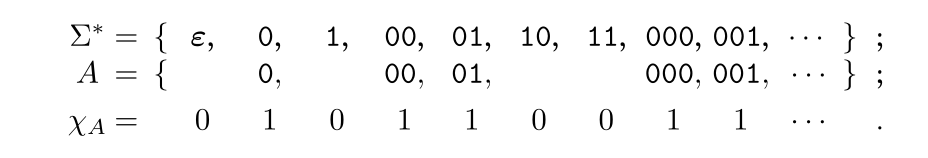
\includegraphics[scale=0.3]{figur/karsekv.png}
		      \end{center}
	\end{itemize}
\end{frame}






%%% Local Variables:
%%% mode: latex
%%% TeX-engine: xetex
%%% TeX-command-extra-options: "-shell-escape"
%%% TeX-master: "main"
%%% End:

\chapter{NP-Komplethedsbeviser}

\section{Tidskompleksitet}%
\label{subsec:label}

\begin{definition}
	Lad $M$ være en Deterministisk Turingmaskine som stopper på alle inputs. \textit{Køretiden} eller \textit{tidskompleksiteten} af $M$ er funktionen $f : \mathbb{N} \rightarrow \mathbb{N}$, hvor $f(n)$ er maksimum antal af skridt som $M$ tager på ethvert input af længde $n$.
\end{definition}

Altså hvis køretiden for eksempel er $3n^{2}$ betyder det at $M$ vil tage højest $3n^{2}$ skridt hvor længden af inputtet er $n$.

\begin{definition}
	Lad $f,g : \mathbb{N} \rightarrow \mathbb{R}^{+}$ være funktioner. Vi siger at $f(n) \in O(g(n))$ hvis der eksisterer $c, n_{0} \in \mathbb{Z}_{+}$ således at $\forall n \ge n_{0} : f(n) \le c \cdot g(n)$
\end{definition}

Intuitivt betyder det at $f(n)$ er mindre end eller lig med $O(g(n))$.

\begin{definition}
	Lad $f, g  \in \mathbb{N}  \rightarrow \mathbb{R}^{+}$. Vi siger at $f(n) \in o(g(n))$ hvis $\lim_{n \to \infty} \frac{f(n)}{g(n)} = 0$. Altså, for hvert $c > 0$ eksisterer der et $n_{0} = n_{0}(c)$ hvor $\forall n \ge n_{0} $ $f(n)  < cg(n)$.
\end{definition}

Intuitivt betyder det at $f(n)$ gror meget langsommere end $o(g(n))$.

\begin{definition}
	Lad $t : \mathbb{N} \rightarrow \mathbb{R}^{+}$ være en funktion. Lad tidskompleksitetsklassen \textit{TIME($t(n)$)} være samlingen af alle sprog som er afgørlige i tid $O(t(n))$ af en Deterministisk Turingmaskine.
\end{definition}

Det er vigtigt at bemærke at \textit{TIME($t(n)$)} kun omhandler afgørselsproblemer, altså problemer hvor man kan svare ``Ja'' eller ``Nej'' til, og ikke problemer såsom sortering.

Hvis et problem har både en optimisering og af afgørselsversion, så er kompleksiteten af dem tæt relateret. For eksempel ved Spanning Tree er der Minimum Spanning Tree problemet, som søger at finder et minimumsstørrelses spanning tree. Dog er der også en afgørselsversion der spørger om der er et spanning tree med vægt $\le k$.

Givet $G = ( V,E,w )$ og $k \in \mathbb{N}$  kan vi afgøre om $\langle G , k \rangle $ er et spanning tree med vægt højest $k$ ved at løse minimum spanning ree problemet på $\langle G \rangle $ og sammenligne $w(T^{*})$ med $k$. Dermed $\langle G, k \rangle \in SpT_{k} \iff w(T^{*}) \le k$, hvor $T^{*}$ er et minimum spanning tree af $G$ med vægtfunktion $w$.

Hvis vi kun har en algoritme til at løse afgørselsversionen, kan vi finde optimeringsversionen ved at lade $k$ være minimumsværdien (normalvist 1), og så gå op derfra, altså prøve med $k$ indtil der er en success. Hvis $i-1$ ikke findes, men $i$ gør, så ved vi at $i$ er minimum.

\begin{definition}
	Lad $M$ være en nondeterministisk Turingmaskine som er en afgører. \textit{Køretiden} af $M$ er funktionen $f : \mathbb{N} \rightarrow \mathbb{N}$ hvor $f(n)$ er maksimumsantallet af skridt som $M$ bruger på en gren af dens komputering på et input af længde $n$.
\end{definition}

Det vil altså sige, at det er den gren der går længst ned, hvor, ved en deterministisk Turingmaskine, er det blot den enkelte gren den har til rådighed.

\begin{theorem}
	Lad $t(n)$ være en funktion hvor $t(n) \ge n$. Så har hver $t(n)$-tids Nondeterministisk Turingmaskine en ækvivalent $w^{O(t(n))}$-tids enkeltbånds Turingmaskine.
\end{theorem}

\begin{proof}
	Vi beviste dette tidligere MANGLER
\end{proof}

Alle \textit{rimelige} deterministiske komputeringsmodeller er polynomielt ækvivalente. Det vil altså sige at alle varianter af Turingmaskiner kan konverteres til hinanden i polynomiel tid, og køre i polynomiel tid.

\subsection{Klassen $\mathcal{P}$}%
\label{subsec:label}

\begin{definition}
	Klassen $\mathcal{P}$ er kompleksitetsklassen af alle problemer der kan løses af Deterministiske Turingmaskiner i polynomiel tid.
	\begin{equation}
		\mathcal{P} = \bigcup_k TIME(n^{k})
	\end{equation}
\end{definition}

Man kan tænke på $\mathcal{P}$ som værende klassen af problemer der realistisk set kan løses af en moderne computer.

Når vi laver en kodning af et problem, skal vi ikke bruge unær notation (altså base-1), da dette er eksponentielt større end alle base-$k$, hvor $k \ge 2$.


Følgende er nogle eksempler på problemer der er en del af kompleksitetsklassen $\mathcal{P}$:
\begin{enumerate}
	\item $S_{p}T_{k}$ som var afgørlighedsversionen af $MST$.
	\item $PATH = \{\langle G , s, t \rangle \mid G \text{ er en rettet graf } s, t, \in V(G) \text{ og } \exists (s,t) \text{ vej i } G\}$
	\item Medlemskab af kontekstfrie sprog: $CFL\text{-}MEMBER = \{\langle G , w \rangle \mid G \text{ er en CFG og } w \in L(G)\}$
	      \begin{enumerate}
		      \item Givet $w \in \Sigma^{*}$ og $G$ som en Chomsky Grammatik, ved vi at $S \stackrel{*}{\Rightarrow} w$ $\iff$ der er en afledning på $2|w| - 1$ skridt.
		      \item Vi ved det er afgørligt, da vi bare kan prøve alle $2|w|-1$ afledeninger. Dette er dog ikke polynomielt i $|w|$.
	      \end{enumerate}
\end{enumerate}

Vi vil gerne kigge videre på problemet om CFL-medlemskab. Vi kan gøre dette polynomielt, men ikke med en naiv metode. I stedet bruger vi \textit{dynamisk programmering}.

Hvis vi antager at $w = \varepsilon$, så kan vi acceptere hvis $S \rightarrow \varepsilon$ er i $R$. Vi kan derfor antage at $|w| > 0$, og at vi kan sætte $w$ op således: $w = a_{1}a_{2} \ldots a_{n}$. $n = |w|$ $a_{i} \in \Sigma$.

Vi konstruerer en $n \times n $ matrix $T$, hvor $T_{ij} = \{A \mid A \Rightarrow a_{i}a_{i+1} \ldots a_{j}\}$ efter komputering. Til at starte med er $T_{ii} = \{A \mid A \rightarrow a_{i} \in R\}$. Vi bruger følgende idé: Hvis $A \rightarrow BC$ og $B \Rightarrow a_{i} \ldots a_{j}$ og $C \Rightarrow a_{j+1} \ldots a_{p}$, så tilføjer vi $A$ til $T_{ip}$. Det betyder så at når vi er færdige med at køre algoritmen, hvis $T_{1n}$  indholder symbolet $S$ kan vi svare ``Ja'' givet en instans, og ellers ``Nej''.

\begin{algorithm}
	\caption{\label{alg:dynamiccfl}Dynamisk Programmerings CFL Løsning}
	\begin{algorithmic}[1]
		\FOR{$i \gets 1$ \TO $n$}
		\FOR{$j \gets i$ \TO $n$}
		\STATE $T_{ij} \gets \emptyset$
		\ENDFOR
		\ENDFOR

		\FOR{$i \gets 1$ \TO $n$}
		\STATE $T_{ii} \gets \{ A \mid A \to a_i \in R \}$
		\ENDFOR

		\FOR{$r \gets 1$ \TO $n-1$}
		\FOR{$i \gets 1$ \TO $n-r$}
		\FOR{$k \gets i$ \TO $i+r-1$}
		\FORALL{rule $A \to BC$}
		\IF{$B \in T_{ik}$ \AND $C \in T_{k+1,i+r}$}
		\STATE $T_{i,i+r} \gets T_{i,i+r} \cup \{ A \}$
		\ENDIF
		\ENDFOR
		\ENDFOR
		\ENDFOR
		\ENDFOR

		\IF{$S \in T_{1n}$}
		\STATE accepter
		\ELSE
		\STATE afvis
		\ENDIF
	\end{algorithmic}
\end{algorithm}

I Algoritme~\ref{alg:dynamiccfl} ses algoritmen beskrevet over.

\begin{definition}
	En \textit{verifikator} for et sprog $L$ er en algoritme $A_{L}$ hvor \\$L = \{w \mid \exists \text{ en streng } c \text{ hvor } A_{L} \text{ accepterer input } \langle w, c \rangle \}$
\end{definition}

Køretiden af $A_{L}$ måles i form af $n = |w|$. $A_{L}$ er en polynomiel verifikator hvis den har køretid $O(n^{k})$. Strengen 4c = c(w) er et \textit{certifikat} for $w \in L$. Bemærk at $|c(w)| \le $ køretiden af $A_{L}$.

For eksempel ved hamiltoniansk kreds problemet, er en verifikator en der tjekker om, givet et certifikat som indeholder en ordning af knuder, om disse knuder former en kreds, og om kardinaliteten af certifikatet er lig med antallet af knuder.

\begin{definition}
	Kompleksitetsklassen $\mathcal{NP}$ er klassen hvor problemerne har en verifikator som kører i polynomiel tid:
	\begin{equation}
		\mathcal{NP} = \{ L \mid L \text{ er en verifikator der kører i polynomiel tid}\}
	\end{equation}
\end{definition}

Bemærk dog at $\mathcal{NP}$ originalt står får \textit{Nondeterministisk Polynomielt}. Vi kigger på eksempel ved \textit{Hampath} som er en vej der går gennem alle knuder, og ser hvordan den kan konstrueres af en nondeterministisk Turingmaskine. Husk at ved en vej i en graf er $s$ startknuden og $t$ slutknuden.

\begin{enumerate}
	\item Gæt $n$ tal $i_{1}, i_{2}, \ldots, i_{n}$ hvor $i_{j} \in \{1, \ldots, n\}$
	\item Tjek om der er nogle ens lister ($i_{p} = i_{q}, p \ne q$). Hvis ``Ja'', \textit{afvis} denne gren.
	\item Tjek om $s = v_{i_{1}}$ og om $t = v_{i_{n}}$. Hvis ``Nej'', \textit{afvis} denne gren.
	\item Tjek om $(v_{i_{p}},v_{i_{p+1}})$ er en kant for $p = 1,2, \ldots, n-1$. Hvis ``Ja'' \textit{accepter}, ellers \textit{afvis}.
\end{enumerate}

\begin{theorem}
	\begin{equation}
		L \in NP \iff L \text{ kan afgøres af en nondeterministisk Turingmaskine}
	\end{equation}
\end{theorem}

\begin{proof}
	Lad $L \in NP$ og $A_{L}$ være en \textit{verifikator} for $L$ hvor $A_{L}$ kører i højest $dn^{k}$ tid, for en konstant $d$ på input af længde $n$.

	Den nondeterministiske Turingmaskine kører som følger:
	\begin{enumerate}
		\item Vælg nondeterministisk en streng $c$ således at $|c| \le dn^{k}$
		\item Kør $A_{L}$ på \(\langle w, c \rangle \)
		\item Accepter hvis $A_{L}$ accepterer, ellers \textit{afvis}.
	\end{enumerate}

	Omvendt, antag at $L$ er afgjort af en nondeterministisk Turingmaskine $M$. Vi konstruerer $A_{M}$ på input \(\langle w, c \rangle \):
	\begin{enumerate}
		\item Simulér $M$ på \(\langle w \rangle  \) ved at bruge \( \langle c \rangle \) til at guide os til hvilken gren vi skal bruge.
		\item Hvis denne gren af $M$'s komputering resulterer i $M$ som accepterer $w$, så accepterer $A_{M}$ \(\langle w , c \rangle \), ellers \textit{afvis}.
	\end{enumerate}

	Altså eksisterer der et $c$ hvor $A_{M}$ accepterer \( \langle w , c \rangle \) $\iff$ $M$ accepterer $\langle w \rangle $.
\end{proof}

\section{Polynomielle Reduktioner}%
\label{sec:label}

\begin{definition}
	Lad $A, B$ være sprog over alfabetet \(\Sigma\). En \textit{polynomiel reduktion} fra $A$ til $B$ er en funktion $f : \Sigma^{*} \rightarrow \Sigma^{*}$ således at:
	\begin{enumerate}
		\item $x \in A \iff f(x) \in B$
		\item Der eksisterer et positivt heltal $k = k(A,B)$ hvor $f(x)$ kan udregnes i $O(|x|^{k})$ tid.
	\end{enumerate}
	Hvis en sådan funktion eksisterer, skriver vi $A \le_{p} B$.
\end{definition}

Definitionen på \textit{polynomielle reduktioner} minder meget om \textit{mapping reduktioner} fra beregnelighedsdelen af kurset. Der er dog én meget vigtig forskel: Vi må kun bruge \textit{polynomiel tid} til at udregne funktionen $f$.

\begin{lemma}
	Hvis $A \le_{p} B$ og $B \in \mathcal{P}$ så $A \in \mathcal{P}$.
\end{lemma}

\begin{proof}
	Antag at $A_{B}$ afgører $B$ i tid $O(n^{c})$ og $C_{A \rightarrow B}$ beregner $f$ således atg $x \in A \iff f(x) \in B$ i tid $O(n^{k})$

	\begin{center}
		\begin{tikzpicture}[auto, thick, node distance=2.5cm, >=triangle 60]
			% Nodes
			\node (alpha) at (0,0) {$\alpha$};
			\node (q0) [right of=alpha] {$f(x)$};
			\node (f) [right of=q0] {};
			\node (acc) [right=-0.3cm of f] {\{accept, afvis\}};

			% Labels
			\path[->] (alpha) edge[bend left] node {$C_{A \to B}$} (q0);
			\path[->] (q0) edge[bend left] node {$\mathcal{A}_B$} (f);

		\end{tikzpicture}
	\end{center}

	Altså betyder det at $C_{A \rightarrow B}$ udregner $f$ i tid $O(n^{k})$ og dermed, hvis input $x$ har størrelse $n = |x|$, og $A_{B}$ udregner i $O(n^{c})$ så får vi en algoritme der kører i $O(n^{c})$ køretid på et input af størrelse $|f(x)| \in O(n^{k})$. Altså producerer $A_{B}$ et svar i tid $O(|f(x)|^{c}) = O((n^{k})^{c}) = O(n^{ck})$
\end{proof}

\begin{definition}
	Et sprog $L$ kaldes \textit{$\mathcal{NP}$-Komplet} hvis
	\begin{enumerate}
		\item $L \in \mathcal{NP}$
		\item \(\forall L' \in \mathcal{NP} : L' \le_{p}\)
	\end{enumerate}
\end{definition}

$\mathcal{NP}$-Komplethedsklassen eksisterer udelukkende grundet \textit{Cook-Levin} sætningen, som vi kommer til senere (Kapitel~\ref{chap:cooklevin}). Vi skriver $L \in \mathcal{NPC}$ hvis $L$ er $\mathcal{NP}$-komplet.

\begin{theorem}
	Hvis $L \in \mathcal{NPC}$ og $L \le_{p} \hat{L}$ så $\hat{L} \in \mathcal{NPC}$.
\end{theorem}
\begin{proof}
	Vi viser først grafisk:

	\begin{center}
		\begin{tikzpicture}[auto, thick, node distance=2.5cm, >=triangle 60]
			% Nodes
			\node (alpha) at (0,0) {$L'$};
			\node (q0) [right of=alpha] {$L$};
			\node (f) [right of=q0] {$\hat{L}$};
			\node (one) [gray] at (0,-0.5) {$x$};
			\node (two) [gray, right of=one] {$f(x)$};
			\node (three) [gray, right of=two] {$g(f(x))$};

			\node (time) [TurquoiseGreen] at (1.3, 0) {$O(n^{r})$};
			\node (time) [TurquoiseGreen] at (3.8, 0) {$O(n^{s})$};

			% Labels
			\path[->] (alpha) edge[bend left] node {$f$} (q0);
			\path[->] (q0) edge[bend left] node {$g$} (f);

		\end{tikzpicture}
	\end{center}
	\begin{center}
		\begin{tikzpicture}[auto, thick, node distance=2.5cm, >=triangle 60]
			% Nodes
			\node (alpha) at (0,0) {$x$};
			\node (q0) [right of=alpha] {$g(f(x))$};
			\node (test) [TurquoiseGreen] at (1.0,0) {$O(n^{rs})$};

			% Labels
			\path[->] (alpha) edge[bend left] node {$g \circ f$} (q0);

		\end{tikzpicture}
	\end{center}

	Vi laver altså en reduktion hvor vi først reducerer fra $L'$ til $L$ i tid $O(n^{r})$. Dette producerer et nyt output fra $x$, kaldet $f(x)$, givet en funktion $f$. Derefter reducerer vi fra $L$ til $\hat{L}$ i tid $O(n^{s})$, hvilket giver et nyt output fra $f(x)$ kaldet $g(f(x))$ givet en funktion $g$. Hvis vi sætter disse to tider sammen, får vi en reduktion i tid $O(n^{rs})$. Dette betyder at $x \in L' \iff g(f(x)) \in \hat{L}$. Dermed, $L' \le_{p} \hat{L} \; \forall L' \in \mathcal{NP}$.
\end{proof}


\subsection{Satisfiability}%
\label{subsec:label}

\begin{definition}
	En \textit{boolsk variabel} $x$ tager to værdier: \textit{Sand og Falsk} (T, F). Nogle gange er sand skrevet $1$ og falsk $0$. Negationen af $x$, skrevet $\overline{x}$ er:
	\begin{equation*}
		\overline{x} = \begin{cases}
			\text{sand}  & \text{ hvis } x = \text{ falsk} \\
			\text{falsk} & \text{ hvis } x = \text{ sand}
		\end{cases}
	\end{equation*}
\end{definition}

\begin{definition}
	En sandhedstildeling til en boolsk variabel $x$ er en tildeling af en værdi sand eller falsk til $x$.
\end{definition}

Satisfiability problemet siger, at givet boolske variabler $x_{1}, x_{2}, \ldots, x_{n}$ og klausuler $C_{1}, C_{2}, \ldots, c_{m}$ over \textit{literals} $x_{1}, \overline{x_{1}}, x_{2}, \overline{x_{2}}, \ldots, x_{n}, \overline{x_{n}}$ e.g. $C_{i} = (x_{i_{1}} \lor \overline{x_{i_{2}}} \lor x_{i_{3}} \lor \overline{x_{i_{n}}})$, eksisterer der en sandhedstildeling $\phi : \{x_{1}, x_{2}, \ldots, x_{n}\} \rightarrow \{T, F\}^{n}$ således at $f = C_{1} \land C_{2} \wedge \ldots \wedge C_{m}$ er sand?

Vi forkorter ofte Satisfiability problemet til SAT.

\begin{theorem}
	SAT \(\in \mathcal{NP}\)
\end{theorem}


\begin{proof}
	Certifikatet er blot en sandhedstildeling \(\phi\) således at hver $C_{i}$ evalueres til sand. Givet \(\phi\) kan vi tjekke i time $O(|f|)$ om $f$ er sand under \(\phi\).
\end{proof}

\begin{theorem}
	\label{theo:satinnpc}
	SAT \(\in \mathcal{NPC}\)
\end{theorem}

\begin{proof}
	Dette bevis findes i kapitel~\ref{chap:cooklevin}.
\end{proof}

\subsection{3-SAT}%
\label{subsec:3sat}

SAT er begrænset til at hver klausul har præcis $3$ literals. For eksempel $f = (x_{1} \vee x_{2} \vee x_{3}) \wedge (\overline{x_{1}} \vee x_{2} \vee x_{3}) \wedge (x_{1} \vee \overline{x_{2}} \vee x_{3}) \wedge (x_{1} \vee x_{2} \vee \overline{x_{3}})$. I dette eksempel satisfier \(\phi = \{x_{1}, x_{2}, x_{3}\} \rightarrow \{T, T, T\}\) $f$.

\begin{theorem}
	3-SAT \(\in \mathcal{NPC}\)
\end{theorem}

\begin{proof}
	Vi beviser i NP og reducering.
	\begin{enumerate}
		\item 3-SAT \(\in \mathcal{NP}\) bevises på samme måde som beviset til Sætning~\ref{theo:satinnpc}.
		\item Vi beviser at SAT $\le_{p}$ 3-SAT.
	\end{enumerate}
	Måden vi reducerer på, er ved at vi ændrer på alle klausuler hvis størrelse \textbf{ikke} er lig med 3, og får dem til at blive en eller flere klausuler af længde 3.

	Hvis $|C_{i}| \ge 4$: $C_{i} = (\lambda_{1} \vee \lambda_{2} \vee \lambda_{3} \vee \cdots \vee \lambda_{k}), k \ge 4$ hvor $\lambda_{i}$ er en literal over $\{x_{1}, \ldots, x_{n}, \overline{x_{1}}, \ldots, \overline{x_{n}}\}$. Vi kan antage at både $x_{i}$ og $\overline{x_{i}}$ \textbf{ikke} er en del af klausulen, da dette ville trivielt gøre klausulen satisfiable. I sådan et tilfælde introducerer vi nye variabler: $y_{1}, y_{2}, \ldots, y_{k-3}$ som er private til klausulen $C_{i}$, og så erstatter vi $C_{i}$ i $f$ med:
	\begin{align*}
		X_{i} = (\lambda_{1} \vee \lambda_{2} \vee y_{1}) \wedge (\overline{y_{1}} \vee \lambda _{3} \vee y_{2}) \wedge (\overline{y_{3}} \vee \lambda_{4} \vee y_{3})
		\wedge \\
		\cdots \\
		\wedge
		(\overline{y_{k-4}} \vee \lambda_{k-2} \vee y_{k-3}) \wedge (\overline{y_{k-3}} \vee \lambda_{k-1} \vee \lambda_{k})
	\end{align*}
	Altså starter vi ud med klausulen $(\lambda_{1} \vee \lambda_{2} \vee y_{1})$ hvor vi tager 2 literals fra klausulen $C_{i}$, og derefter følger vi et mønster $(\overline{y_{i}} \vee \lambda_{i+2} \vee y_{i+1}) \wedge (\overline{y_{i+1}} \vee \lambda_{i+3} \vee y_{i+2})$, hvor $i = 1 \ldots k-5$ ($k-5$ da jeg bruger eksemplet op til $i+2$) indtil vi når til den sidste klausul hvor det er $(\overline{y_{k-3}} \vee \lambda_{k-1} \vee \lambda_{k})$.

	\begin{claim}
		$X_{i}$ er sand $\iff$ mindst én af $\lambda_{j}$ er sand $j \in 1 \ldots k$
	\end{claim}

	\begin{proof}
		\(\Leftarrow\)\\
		\noindent
		Hvis vi sætter alle $y_{i}, i = 1 \ldots k-3$  undtagen den $y_{z}$  som fremstår unegeret i den klausul som én \(\lambda\) er sand i. Dermed er alle klausuler sande, inklusiv den ene, hvor \(\lambda\) er den eneste sande værdi, da $\overline{y_{j-1}}$ er falsk, men \(\lambda_{j+1}\) er sand, og da $y_{j}$ er falsk, betyder det også at den næste klausul vil være sand, da den har en negering, og resten vil være sande, da vi satte alle andre til at være sande.\\\\
		\noindent
		\(\Rightarrow\)\\
		\noindent
		Hvis vi antager at alle $\lambda_{i}$ er falske, så ville vi være nødt til at sætte alle $y_{j}$ til at være sande. Problemet er dog at grundet vores sidste klausul, som ikke indeholder en u-negeret $y$ literal, ville blive falsk. Det er også derfor den anden vej virker, på et eller andet tidpsunkt skal $y$--erne skifte til at blive falske, og så er én af $\lambda$'erne nødt til at være sande i den klausul, da der ikke kan være 3 negative i $f$, da dette ville gøre den falsk.\footnote{Dette er meget svært at forklare. Jørgen er inde over det omkring 27 minutter inde i video 16.}
	\end{proof}
\end{proof}



%%% Local Variables:
%%% mode: latex
%%% TeX-engine: xetex
%%% TeX-command-extra-options: "-shell-escape"
%%% TeX-master: "main"
%%% End:

\section{Cook-Levin}%
\label{sec:cooklevin}

\begin{frame}
	\frametitle{Pensum}
	\begin{itemize}
		\item Sipser 7.4: \textbf{Bevis at CNF-SAT er NP-Komplet}
		\item Weekly Note 9
		\item Video 18 (Bonus \href{https://www.youtube.com/watch?v=6Az1gtDRaAU}{video})
	\end{itemize}
\end{frame}

\begin{frame}[allowframebreaks]
	\frametitle{Cook-Levin}
	\begin{definition}
		$B$ er $NP$-komplet hvis:
		\begin{enumerate}
			\item $B \in NP$
			\item $\forall A \in NP, A \le_{P} B$
		\end{enumerate}
	\end{definition}
	\begin{itemize}
		\item Man antager generelt at $P \ne NP$, så derfor hvis vi beviser NP-Komplethed for et problem, beviser vi at der nok ikke er en polynomiel algoritme der kan løse problemet.
	\end{itemize}

	\begin{center}
		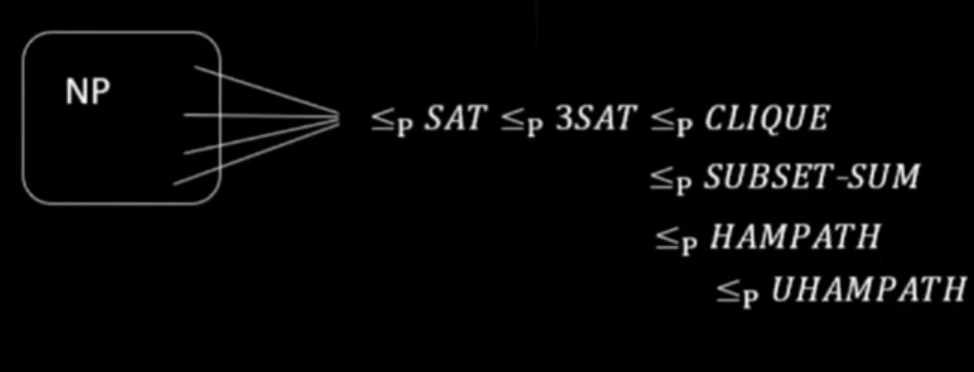
\includegraphics[scale=0.4]{figur/video16a.png}
	\end{center}

	\begin{itemize}
		\item Reminder: \(\sum_{1 \le i \le n}i = 1 + 2+ \cdots + n\)
		\item På samme måde hvis $x = x_{1} \cdots x_{n}$ og $y = y_{1} \cdots y_{n}$, hvornår gælder følgende så?
		      \begin{equation}
			      \left( \bigwedge_{1 \le i \le n} x_{i} = y_{1} \right) = True
		      \end{equation}
		\item Svar: Når $x = y$!
		\item Altså bliver den til udtrykket $(x_{1} = y_1) \land (x_{2} = y_2) \land \cdots \land (x_{k} = y_{k})$
		\item Til gengæld, hvis det var følgende udtryk i stedet:
		      \begin{equation}
			      \left( \bigvee_{1 \le i \le n} x_{i} = y_{1} \right) = True
		      \end{equation}
		\item Ville svaret være når $x_{i} = y_{i}$ for en eller anden $i$.
		\item Nu er vi ved at være klar!
	\end{itemize}

	\begin{theorem}
		$SAT$ er $NP$-komplet.
	\end{theorem}
	\begin{itemize}
		\item Jeg bruger (sandsynligvis) udelukkende Sipsers \href{https://youtu.be/6Az1gtDRaAU}{video forelæsning}. Det vil sige at hverken Jørgens noter, eller bogen er brugt til dette.
		\item Beviset er faktisk ikke så svært! Det er bare meget langt.
		\item For at bevise sætningen, skal vi bevise to ting:
		      \begin{enumerate}
			      \item $SAT \in NP$ (allerede gjort, hvis ikke bliver det gjort i spørgsmål 5 når jeg er færdig med den.)
			      \item $\forall A \in NP : A \le_{P} SAT$.
		      \end{enumerate}

		\item Givet en $A \in NP$ som afgøres af en NDTM i tid $n^{k}$ altså polynomiel.
		\item Vores mål er at give en reduktion i polynomiel tid $f$ som mapper $A$ til $SAT$.
		\item Måden denne fungerer på er ved at mappe strenge som \textit{måske} er i $A$ til sandhedsformler som \textit{måske} er satisfiable.
		\item $f : \Sigma^{*} \longrightarrow \text{ formler }$
		\item $f(w) = \langle \phi_{M,w} \rangle$
		\item $w \in A \iff \phi_{M,w}$ er satisfiable.
		\item Så altså er vores mål at lave en reduktion der reducerer så en streng er i $A$ \textbf{hvis og kun hvis} den resulterende formel er satisfiable.
		\item Vores idé er at lade $\phi_{M,w}$ \textit{simulere} $M$ på $w$, så vi designer \(\phi_{M,w}\) til at ``sige'' at $M$ accepterer $w$.
		\item Så man kan se \(\phi_{M,w}\) som et statement: ``$M$ accepterer $w$'', og resultatet er så enten \textit{sandt} eller \textit{falsk}.
	\end{itemize}

	\begin{definition}
		En (accepterende) tableau for en NDTM $M$ på $w$ er en tabel af størrelse $n^{k} \times n^{k}$, som repræsenterer en \textit{komputeringshistorie} for $M$ på $w$ på en accepterende gren af den nondeterministiske komputering.
	\end{definition}
	\begin{center}
		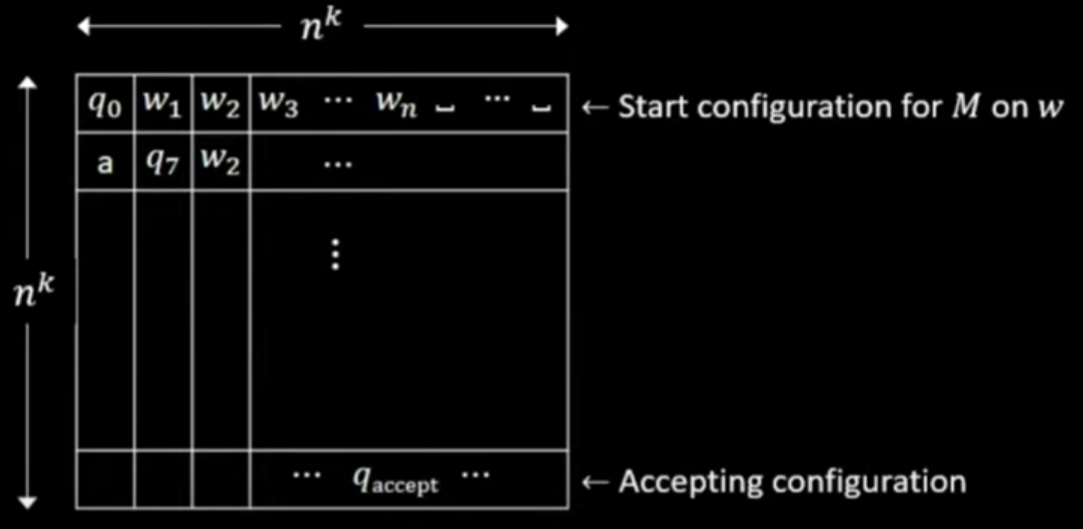
\includegraphics[scale=0.45]{figur/video16b.png}
	\end{center}

	\begin{itemize}
		\item Det betyder altså at denne tableau er en ``historie'' for hvordan $M$ kører på $w$ og accepterer $w$.
		\item Hver række er altså en konfiguration af maskinen.
		\item Række 2 viser altså en mulig næste konfiguration hvor den næste tilstand er $q_{7}$, den er rykket én til højre, og har ændret $w_{1}$ til $a$.
		\item Størrelsen på tabellen kommer fra at maskinen har køretid $n^{k}$, så dermed kan den højest køre i $n^{k}$ skridt, og højest lave $n^{k}$ ændringer på båndet.
		\item Det er \textbf{vigtigt} at huske at en tableau kun er én accepterende gren, ikke alle grene!
		\item Vores mål er nu at konstruere \(\phi_{M,w}\) til at ``sige'' at $M$ accepterer $w$, og altså dermed sige at der eksisterer en tableau $M$ på $w$.
		\item Husk at vi her antager at en tableau er \textit{accepterende}.
		\item Måden vi kommer til at konstruere denne formel på er i skridt, som følger: \(\phi_{M,w} = \phi_{cell} \land \phi_{start} \land \phi_{move} \land \phi_{accept}\)
		\item Så altså siger \(\phi_{M,w}\) at:
		      \begin{enumerate}
			      \item \(\phi_{cell}\): Cellerne er korrekte
			      \item \(\phi_{start}\): Den starter korrekt
			      \item \(\phi_{move}\): Den bevæger sig korrekt
			      \item \(\phi_{accept}\): Den ender korrekt
		      \end{enumerate}
		\item Bare rolig, det er ikke meningen at noget af dette skal give mening endnu.
	\end{itemize}
\end{frame}

\begin{frame}[allowframebreaks]
	\frametitle{Konstruktion af \(\phi\): \(\phi_{cell}\)}
	\begin{center}
		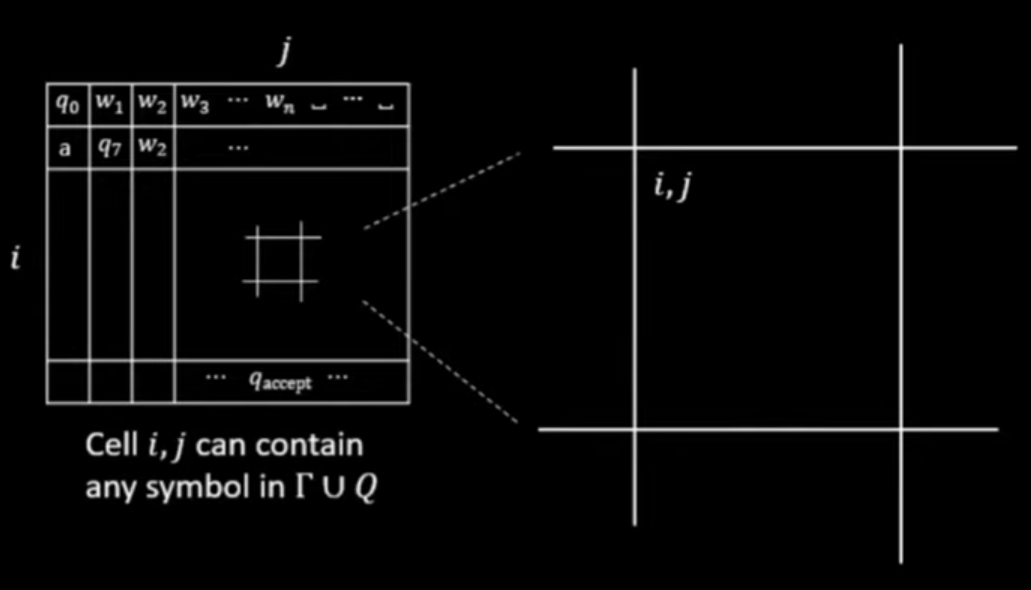
\includegraphics[scale=0.3]{figur/video16c.png}
	\end{center}
	\begin{itemize}
		\item Variablerne i \(\phi_{M,w}\) er $x_{i,j,\sigma}$ for $1 \le i,j \le n^{k}$ og $\sigma \in \Gamma \cup Q$
		\item Det vil altså sige at der er en variabel for én af hvert symbol $\sigma \in \Gamma \cup Q$.
	  \item Dette er fordi, en konfiguration er en blanding af båndsymboler og tilstande.
		\item Hvis $x_{i,j,\sigma} = \text{\texttt{True}}$, betyder det at cellen $i,j$ indeholder symbolet \(\sigma\).
	  \item Så, hvis $i,j$ indholder $a$, så vil $x_{i,j,a} = True$, men $x_{i,j,\sigma}$ hvor $\sigma = (\Gamma \cup Q) \setminus \{a\}$ ville være falsk.
	  \item Det introducerer altså en regel: Hver celle må \textbf{højest} have én sand værdi.
	  \item På samme tid, trods der kun må være én sand værdi, skal det også \textbf{mindst} være en sand værdi!
	  \item Måden vi sikrer at der mindst er en sand værdi:
			\begin{equation}
x_{i,j,\sigma_{1}} \lor x_{i,j,\sigma_{2}} \lor \cdots \lor x_{i,j,\sigma_{t}}
			\end{equation}
	  \item Som vi kan skrive således:
			\begin{equation}
\bigvee_{\sigma \in \Gamma \cup Q} x_{i,j,\sigma}
			\end{equation}
	  \item Vi vil også sikre at er \textit{højest} er én sand variabel:
			\begin{equation}
\bigwedge_{\sigma, \tau \in \Gamma \cup Q, \sigma \ne \tau} (\overline{x_{i,j,\s} \land x_{i,j,\tau}})
			\end{equation}

	  \item Altså for alle to forskellige symboler, \(\sigma\) og \(\tau\) må de \textbf{ikke} være sande.
	  \item Måden vi får en formel der kigger for begge disse, er bare ved at putte dem sammen via en $\lor$ operation, således:
			\begin{equation}
\left(  \bigvee_{\sigma \in \Gamma \cup Q} x_{i,j,\sigma} \right) \land \left(    \bigwedge_{\sigma, \tau \in \Gamma \cup Q, \sigma \ne \tau} (\overline{x_{i,j,\s} \land x_{i,j,\tau}}) \right)
			\end{equation}
	  \item Vi vil gerne have at denne operation skal laves over \textit{alle} mulige celler:
			\begin{equation}
\bigwedge_{1 \le i,j \le n^{k}} \left( ... \right)
			\end{equation}
	  \item Så vi ender altså med en formel for \(\phi_{cell}\) som følger:
			\begin{equation}
			  \bigwedge_{1 \le i,j \le n^{k}} \left(
\left(  \bigvee_{\sigma \in \Gamma \cup Q} x_{i,j,\sigma} \right) \land \left(    \bigwedge_{\sigma, \tau \in \Gamma \cup Q, \sigma \ne \tau} (\overline{x_{i,j,\s} \land x_{i,j,\tau}}) \right)
			  \right)
			\end{equation}
	\end{itemize}
\end{frame}

\begin{frame}
  \frametitle{Konstruktion af \(\phi\): \(\phi_{start}\), \(\phi_{accept}\)}
\begin{itemize}
  \item I sin essens:
		\begin{itemize}
		  \item \(\phi_{start}\) siger at startkonfigurationen skal være $q_{0}w_{1}\ldots w_{n} \sqcup \ldots \sqcup$
		  \item \(\phi_{accept}\) siger at den sidste konfiguration skal være en valid acceptkonfiguration $ \cdots q_{accept} \cdots$.
		\end{itemize}

  \item Måden vi laver \(\phi_{start}\) på er simpelt:
		\begin{equation}
\phi_{start} = x_{1,1,q_{0}} \wedge x_{1,2,w_{1}} \wedge \cdots \wedge x_{1,n+1,w_{n}} \wedge \cdots \wedge x_{1,n^{k}, \sqcup}
		\end{equation}
  \item \(\phi_{accept}\) er på samme måde meget simpelt:
		\begin{equation}
\bigvee_{1 \le j \le n^{k}} x_{n^{k}},j,q_{accept}
		\end{equation}

  \item Altså skal bare én af disse være $q_{accept}$.
\end{itemize}
\end{frame}

\begin{frame}[allowframebreaks]
  \frametitle{Konstruktion af \(\phi\): \(\phi_{move}\)}
\begin{itemize}
  \item \(\phi_{move}\) skal sikre sig at hver ændring af konfigurationen fra et skridt til det næste, er lovligt.
  \item Måden vi gør dette på er ved at bruge ``neighbourhoods'' eller ``nabolag'', som er $2\times3$ celler i tableauen.
		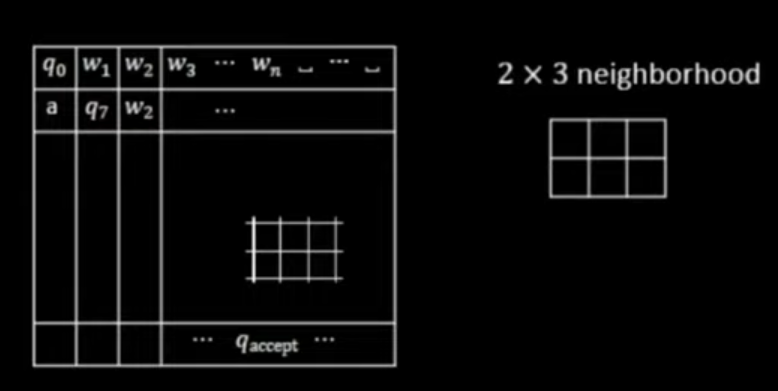
\includegraphics[scale=0.4]{figur/video16d.png}
  \item Move er i sin essens relativt simpelt: Hvis alle 3 celler er lovlige, og vi går igennem alle mulige neighbourhoods, så er hele bevægelsen lovlig.
  \item Følgende er eksempler på lovlige og ulovlige nabolag:
		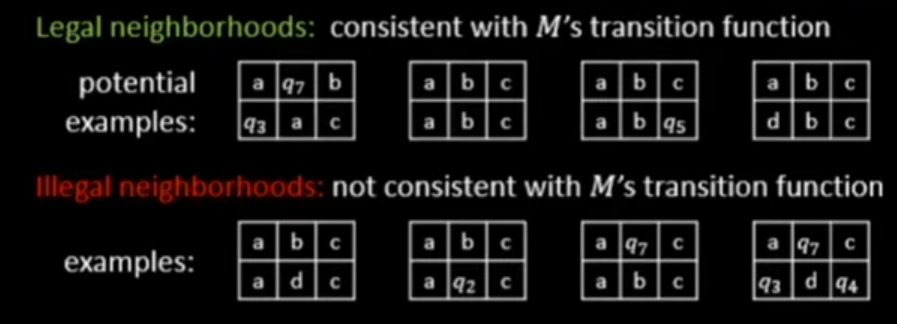
\includegraphics[scale=0.4]{figur/video16e.png}

  \item \textbf{Spørgsmål}: Hvorfor er den sidste ulovlig, når det er en NDTM?
  \item Det sidste eksempel er også grunden til at et $2 \times 2$ nabolag ikke er nok.
  \item Vi laver så dette til en boolsk formel, givet et nabolag $((r,s,t),(v,y,z))$:
		\begin{equation}
\bigvee_{Lovlig}  (x_{i,j-1,r} \wedge x_{i,j,s} \wedge x_{i,j+1,t} \wedge x_{i+1,j-1,v} \wedge x_{i+1,j,y} \wedge x_{i+1,j+1,z})
		\end{equation}
  \item Vi vil så gerne gøre dette for alle mulige $i,j$ så vi ved at hele tableauen's overføringsfunktion er korrekt:
		\begin{align*}
		  \phi_{move} = \bigwedge_{1 < i,j < n^{k}}& \Big( \bigvee_{Lovlig} (x_{i,j-1,r} \wedge x_{i,j,s} \wedge  \\
		  &x_{i,j+1,t} \wedge x_{i+1, j-1, v} \wedge x_{i+1,j,y} \wedge x_{i+1,j+1,z}) \Big)
		\end{align*}
  \item Bemærk her at $\bigvee_{Lovlig}$ betyder at den tager alle lovlige nabolag, og ser om det er en af dem.
  \item Der er kun en endelig del af disse, $|\Gamma \cup Q|^{6}$.
  \item Til sidst: Vi kigger på noterne vi må bruge til eksamen, og ``oversætter''.
\end{itemize}
\end{frame}

%%% Local Variables:
%%% mode: latex
%%% TeX-engine: xetex
%%% TeX-command-extra-options: "-shell-escape"
%%% TeX-master: "main"
%%% End:

\chapter{Pumpelemmaet for regulære og kontekstfrie sprog}



%%% Local Variables:
%%% mode: latex
%%% TeX-engine: xetex
%%% TeX-command-extra-options: "-shell-escape"
%%% TeX-master: "main"
%%% End:

\chapter{Informationsteoretiske Nedre Grænser og Modstander Nedre Grænser for sortering ved sammenligninger}

\section{En $\Omega (n \log n)$ nedre grænse til sortering ved sammenligninger}%
\label{sec:sorteringsalgoritmesammenligninger}

\begin{note}[Kilder]
Video 24 \\
\href{https://imada.sdu.dk/u/jbj/DM553/LBnoteJBJ21.pdf}{Kapitel 7 - Jørgens noter til nedre grænser}
\end{note}

Vores mål her er at vise at en modstander altid vil kunne tvinge $\frac{1}{2}n \log n$ sammenligninger i enhver sammenligningsbaseret sorteringsalgoritme. Vi antager at listen der skal sorteres har størrelse $n$, og at $n = 2^{k}$, for et ikke-negativt heltal $k$.Modstanderen har, til at lave sin strategi, et binært træ $T$ af dybde $k = \log n$, hvis knuder indeholder elementer. Til at starte med er det kun roden i træet, hvis størrelse ikke er 0, den indeholder nemlig de $n$ elementer der skal sorteres.

Vi giver træet ``niveauer'', sålede at niveau 0 indeholder roden, og niveau $\ell$ indeholder $2^{\ell}$ ``poser''.\footnote{Poser er en anden måde at sige knuder på, vi bruger poser til at betyde knuder der kan indeholde elementer.} Et deltræ $T[b]$ er et deltræ hvor roden er knuden $b$. Ethvert deltræ $T[b]$ på niveau $\ell$ har den invariant, at størrelsen $|T[b]| \le 2^{k-\ell} = \frac{n}{2^{\ell}}$.\footnote{Invariant betyder at udsagnet som følger holder igennem hele algoritmen.}

I algoritmen som modstanderen bruger når vedkommende svarer på en sammenligning, bevæger hvert element sig ned igennem træet, indtil alle $n$ elementer er i deres egen private pose, af størrelse $1$ på niveau $k-1$.\footnote{$k-1$ fordi roden er niveau $0$ og dybden er $k$.} Når dette sker, er alle elementerne sorteret.

Vi definerer tre tilstande, som en pose $b$ kan være i igennem køringen af algoritmen:
\begin{itemize}
  \item \textbf{Åben}: Både venstre og højre deltræ af $b$  har mindre end $2^{k-\ell-1}$ elementer.
  \item \textbf{Højre-flushed}: Venstre deltræ har størrelse $2^{k-\ell-1}$.
  \item \textbf{Venstre-flushed}: Højre deltræ har størrelse $2^{k-\ell-1}$.\footnote{Jørgens noter har nogle fejl i, som han ikke forklarer i videoen. Jeg har valgt at sige at ``venstre-flush'', betyder at elementerne kan komme ned til venstre deltræ. Derudover forklarer han slet ikke i noterne hvad hhv. right og left-flush er, han antager bare at man ved det.}
\end{itemize}

I Figur~\ref{fig:flushes} ses de tre tilstande for en pose $b$.

\begin{figure}[ht]
\centering
\begin{tikzpicture}[level distance=2cm, sibling distance=2.5cm, every node/.style = {shape=rectangle, draw, align=center}]
% Open state
\node at (-4,0) {$b$ er åbent} [sibling distance=2.0cm]
child {node {$<2^{k-\ell-1}$}}
child {node {$<2^{k-\ell-1}$}};

% Left-flushed state
\node at (0,0) {$b$ er højre-flushed} [sibling distance=2.0cm]
child {node {$=2^{k-\ell-1}$}}
child {node {$<2^{k-\ell-1}$}};

% Right-flushed state
\node at (4,0) {$b$ er venstre-flushed} [sibling distance=2.0cm]
child {node {$<2^{k-\ell-1}$}}
child {node {$=2^{k-\ell-1}$}};
\end{tikzpicture}
  \caption{\label{fig:flushes} De 3 tilstande $b$ kan være i.}
\end{figure}

Til at udføre sin strategi, gør modstanderen brug af følgende funktioner:
\begin{itemize}
  \item \textbf{MOVE(u)}: Denne funktion kaldes når et element $u$ er kommet til posen $b'$, og gør som følger:
        \begin{itemize}
          \item Hvis $b'$ er \textbf{åbent} forbliver $u$ i $b'$.
          \item Hvis $b'$ er \textbf{højre-flushed} eller \textbf{venstre-flushed} bliver elementet $u$ flyttet til posen $b'$ på hhv. højre eller venstre deltræ. Derefter bliver \textbf{MOVE(u)} kaldt igen.
        \end{itemize}
  \item \textbf{CHECK(u)}: Denne funktion kaldes ved en åben pose $b$, og gør som følger:
        \begin{itemize}
          \item Tjekker om enten højre eller venstre deltræ $T[b]$ af posen $b$ på niveau $\ell$ indeholder $2^{k-\ell-1}$ elementer, og hvis så, markerer den pose $b$ hhv. venstre eller højre-flushed.
          \item Kalder \textbf{MOVE} på \textit{alle} elementer i $b$.
        \end{itemize}
\end{itemize}

I Algoritme~\ref{alg:move} og Algoritme~\ref{alg:check} kan algoritmiske fortolkninger ses af hhv. CHECK og MOVE.

\begin{algorithm}
\caption{\label{alg:move} MOVE(u)}
\begin{algorithmic}[1]
\STATE $b(u)$ \COMMENT{Nuværende pose af $u$}
\IF{$b(u)$ er åben}
    \RETURN
\ELSIF{$b(u)$ er venstre-flushed}
    \STATE $b(u) \gets b^L(u)$
    \STATE MOVE($u$)
    \RETURN
\ELSIF{$b(u)$ er højre-flushed}
    \STATE $b(u) \gets b^R(u)$
    \STATE MOVE($u$)
    \RETURN
\ENDIF
\end{algorithmic}
\end{algorithm}

\begin{algorithm}
\caption{\label{alg:check} CHECK(b)}
\begin{algorithmic}[1]
\STATE $b$ er en åben pose på niveau $\ell$
\IF{$|T[b^R]| = 2^{k-\ell-1}$}
    \STATE Marker $b$ som venstre-flushed \COMMENT{højre undertræ er fyldt}
    \STATE MOVE($u$)
    \RETURN
\ENDIF
\IF{$|T[b^L]| = 2^{k-\ell-1}$}
    \STATE Marker $b$ som højre-flushed \COMMENT{venstre undertræ er fyldt}
    \STATE MOVE($u$)
    \RETURN
\ENDIF
\RETURN
\end{algorithmic}
\end{algorithm}

\subsection{Modstanderens Strategi}%
\label{subsec:label}

Imens modstanderen svarer på spørgsmål om $x < y$ fra algoritmen, så flytter den enten 2, 1, eller 0 elementer ned i træet, men \textbf{en undtagelse}: Efter hvert \textit{MOVE(u)} kald på et element $u$ fra posen $b$, kalder vi \textit{CHECK(b)}, som kan flytte op til $2^{k-\ell -1}$ elementer. Efter hver query som resulterer i at mindst et element flyttes, kaldes \textit{MOVE(u)} rekursivt på elementet.

Antag at sorteringsalgoritmen $A$ efterspørger resultatet på en sammenligning af elementer $u$ og $v$. Lad \(\ell(u)\) og \(\ell(v)\) være niveauene af hhv. $l$ og $v$. Lad $b(u)$ og $b(v)$ være poserne der indeholder henholdvis $u$ og $v$.

\begin{enumerate}
  \item Hvis den mindste fælles forfader (least comon ancestor) $b$ af $b(u)$ og $b(v)$ i $T$ ikke er $b(u)$ eller $b(v)$, så svarer modstanderen ``$u < v$'' hvis $u$ er i det venstre undertræ af $b$ og $v$ i det højre, og ``$v < u$'', hvis $u$ er i det højre undertræ af $b$ og $u$ i det venstre. Intet element flyttes her. $A$ får ingen information ud af den her sammenligning.
  \item Hvis den mindste fælles forfader $b$ af $b(u)$ og $b(v)$ er i $\{b(u), b(v)\}$, så kan man, uden tab af generalitet, sige at $b = b(u)$ eller $b = b(v)$. Vi antager herfra at $b = b(u)$.
\end{enumerate}





%%% Local Variables:
%%% mode: latex
%%% TeX-engine: xetex
%%% TeX-command-extra-options: "-shell-escape"
%%% TeX-master: "main"
%%% End:

\section{Adversary Argumenter}%
\label{sec:adversaryargumenter}

\begin{frame}
  \frametitle{Pensum}
  \begin{itemize}
    \item Baase 3: \textbf{Adversary nedre grænse argumenter}
    \item Baase 3.5: \textbf{Adversary Median Problem}
    \item Jørgens noter: \textbf{Noter på nedre grænser}
    \item Weekly Note 12
    \item Video 24-25
  \end{itemize}
\end{frame}



%%% local variables:
%%% mode: latex
%%% tex-engine: xetex
%%% tex-command-extra-options: "-shell-escape"
%%% tex-master: "main"
%%% end:

\section{Algoritmer med faste parametre}%
\label{sec:algoparametre}

\begin{frame}
  \frametitle{Pensum}
  \begin{itemize}
    \item Cygan et al pp. 3-8, 12-14, 17--22, 51-55: \textbf{Algoritmer med faste parametre}.
    \item F.V. Fomin, D. Kratsch pp. 1-6: \textbf{Eksakte Algoritmer}.
    \item Weekly Note 13
    \item Video 26
  \end{itemize}
\end{frame}

\begin{frame}{Introduktion}
    Antag at du er ejer af en bar. Du skal sørge for at der ikke kommer nogen slåskampe.
    \begin{itemize}
        \item Du kender allerede de personer der gerne vil slås, og hvem de gerne vil slås med.
        \item Dit mål er derfor at, givet $n$ personer, vil du gerne ekskludere $k$ personer, således at så få personer som muligt kommer op og slås.
    \end{itemize}
\end{frame}

\begin{frame}{Vertex-Cover Problem}
    \begin{itemize}
        \item Vi kan modellere dette som et problem af \textsc{Vertex-Cover} problemet.
        \item Her er en knude en person, og en kant mellem to knuder betyder at de to knuder vil slås.
    \end{itemize}
\end{frame}

\begin{frame}{Eksempel på en graf}
    \begin{figure}
        \centering
        \begin{tikzpicture}[scale=0.5]
            \begin{scope}[every node/.style={circle,thick,draw}]
                \node (A) at (0,0) {};
                \node (B) at (0,3) {};
                \node (C) at (2.5,4) {};
                \node (D) at (2.5,1) {};
                \node (E) at (2.5,-1) {};
                \node (F) at (5,2) {};
            \end{scope}
            \begin{scope}[>={Stealth[black]}]
                \path [-] (A) edge node {} (B);
                \path [-] (A) edge node {} (D);
                \path [-] (D) edge node {} (C);
                \path [-] (D) edge node {} (E);
                \path [-] (D) edge node {} (F);
                \path [-] (E) edge node {} (F);
            \end{scope}
        \end{tikzpicture}
        \caption{\label{fig:barfightvertexcover} En graf $G = (V,E)$.}
    \end{figure}
    \begin{itemize}
        \item I Figur~\ref{fig:barfightvertexcover} ses et eksempel på en normal graf.
        \item Hver knude en person, og hver kant mellem to knuder, en slåskamp der venter på at ske.
    \end{itemize}
\end{frame}

\begin{frame}{Barkampsproblemet}
    \begin{itemize}
        \item Vi skal løse barkampsproblemet, men da \textsc{Vertex-Cover} er $\mathcal{NP}$-komplet, kan vi ikke bare gøre det som normalt.
        \item Der er to umiddelbare metoder: \textit{Den Naive Metode} og \textit{Binomialmetoden}.
    \end{itemize}
\end{frame}

\begin{frame}{Naive og Binomialmetoder}
    \begin{itemize}
        \item Naive Metode: Prøver alle $2^{1000} \approx 1.07 \cdot 10^{301}$ delmængder.
        \item Binomialmetoden: Prøver alle $\binom{n}{k}$ delmængder af størrelse $k$, hvilket er cirka $2.63 \cdot 10^{23}$ muligheder.
    \end{itemize}
\end{frame}

\begin{frame}{Problemreducering og Kernelisering}
    \begin{itemize}
        \item Vores løsning til problemet er at tage instansen og give det nogle regler, som vi kalder "sikkerhedsregler".
        \item Disse regler sikrer et mindre input, som vi så kan arbejde med.
    \end{itemize}
\end{frame}

\begin{frame}{Regler for Vertex-Cover}
    Givet en graf $G = (V,E)$ og et ikke-negativt heltal $k$:
    \begin{itemize}
        \item \textbf{Regel 1}: Hvis $\forall v \in V \mid d(v) = 0$, så fjerner vi $v$ fra grafen.
        \item \textbf{Regel 2}: Hvis $\forall v \in V \mid d(v) \ge k + 1$ så fjerner vi $v$ og reducerer $k$ med én.
        \item \textbf{Regel 3}: Hvis $\forall v \in V \mid d(v) = 1 \text{ og } w \text{ er den eneste nabo til }v$ så fjerner vi $v$ og $w$ i grafen, og reducerer $k$ med 1.
    \end{itemize}
\end{frame}

\begin{frame}{Reduktion og Kernelisering}
    \begin{itemize}
        \item Vi putter disse regler på inputtet $G$ indtil ingen af dem er mulige længere.
        \item Hvis $k' = 0$ og der stadig er kanter i grafen, så kan vi afvise $(G, k)$.
    \end{itemize}
\end{frame}

\begin{frame}{Eksempel på Kernelisering}
    \begin{itemize}
        \item Hvis $|E'| \le k'^{2}$ og $|V(G')| \le k^{2}$.
        \item Vi får dette resultat fra følgende udregning:
    \end{itemize}
    \begin{equation*}
        |V'| = \sum_{v \in V'} 1 = \frac{1}{2} \sum_{v \in V'} 2 \le \frac{1}{2} \sum_{v \in V'} d(v) = |E'| \le k'^{2} \le k^{2}
    \end{equation*}
\end{frame}

\begin{frame}{Brute-Force Algoritme}
    \begin{itemize}
        \item Når vi har sat disse regler ind og udført dem, kan vi køre en brute-force algoritme på inputtet $(G', k')$.
        \item Hvis $k = 10$ betyder det at vi højest skal prøve $\binom{100}{10} \approx 1.73 \cdot 10^{13}$ mulige delmængder.
    \end{itemize}
\end{frame}

\begin{frame}{Tid på Kernelisering}
    \begin{itemize}
        \item Tiden der bliver brugt i kerneliseringen af inputtet er $O((n+m)k)$.
        \item Hvis vi ikke afviser instansen, så kommer vi til en instans $(G', k')$.
    \end{itemize}
\end{frame}

\begin{frame}{Definitioner}
    \begin{itemize}
        \item \textbf{Parameteriseret Problem}: Et \textit{parameteriseret problem} $Q$ er \textit{Fastsat Parameter Traktabel} (FPT) hvis der eksisterer en algoritme $A_{Q}$ der løser $Q$ i tid $O(f(k) \cdot n^{c})$ for en beregnlig funktion $f$ og en konstant $c \in \mathbb{R}_{+}$.
        \item \textbf{Kernelisation, kernel}: En kernelisationsalgoritme (en kernel) for et parameteriseret problem $Q$ er en algoritme $A_{Q}$, som, givet en instans $(I,k)$ kører i polynomiel tid i $|(I,k)|$ og outputter en ækvivalent instans $(I', k')$, hvor $|I'| + k' \le g(k)$ for hver instans $(I, k)$ af $Q$ og $g$ er en fastsat beregnelig funktion.
    \end{itemize}
\end{frame}

\begin{frame}{Kernel til Vertex-Cover}
    \begin{itemize}
        \item Ved \textsc{Vertex-Cover} problemet, tog vi input $(G, k)$ og producerede en kernel $(G', k')$ som opfylder kravet $|G'| + k' \le 2k^{2} + k$.
    \end{itemize}
\end{frame}

\begin{frame}{En kernel af størrelse højest $2k$ til \textsc{Vertex-Cover}}
    \begin{itemize}
        \item I delkapitel så vi den følgende approximationsalgoritme baseret på lineær programmering for \textsc{Vertex-Cover}.
    \end{itemize}
    \begin{enumerate}
        \item Løs $Z_{LP} = \min \sum_{v \in V} X(v)$ således at $X(u)+X(v) \ge 1 \; \forall (u,v) \in E$ og $0 \le X(u) \le 1$.
        \item Lad $\hat{X}$ være en optimal LP-løsning.
        \item Tag $U = \{v \mid \hat{X}(v) \ge \frac{1}{2}\}$
    \end{enumerate}
\end{frame}

\begin{frame}{Nemhauser-Trotter Sætning}
    \begin{itemize}
        \item Der eksisterer et optimalt vertex-cover $U^{*}$ således at $V_{>} \subseteq U^{*} \subseteq V_{=} \cup V_{>}$.
        \item Bevis: Antag at $X$ er et optimal vertex-cover af $G = (V,E)$ og at $X \cap V_{<} \ne \emptyset$.
    \end{itemize}
\end{frame}

\begin{frame}{Lad $k^{*} = |U^{*}|$}
    \begin{itemize}
        \item Husk at vi kan antage at $V_{>} \subseteq U^{*}$.
        \item Lad $G' $ være delgrafen af $V_{=}$, og lad $k' = k - |V_{>}|$.
    \end{itemize}
\end{frame}

\begin{frame}{Tilbage til Barkampsanalogien}
    \begin{itemize}
        \item Først løser vi det lineære programmeringsproblem.
        \item Så finder vi $V_{<}, V_{=}$ og $V_{>}$.
        \item Hvis $|V_{>}| \ge k$ afviser vi.
    \end{itemize}
\end{frame}

\begin{frame}{Træsøgning}
    \begin{itemize}
        \item Vi vil nu vise hvordan man kan løse bedre end brute-force.
        \item Givet en instans $(G,k)$, prøv kanterne i en eller anden ordning.
    \end{itemize}
    \begin{figure}
        \centering
        \begin{tikzpicture}[level distance=1.5cm,
                level 1/.style={sibling distance=3cm},
                level 2/.style={sibling distance=1.5cm}]
            \node {a-b}
            child {node {b-c}
                    child {node {c-d}}
                    child {node {b-d}}
                }
            child {node {c-d}
                    child {node {d-e}}
                    child {node {e-f}}
                };
        \end{tikzpicture}
        \caption{\label{fig:treesearchvc} Træsøgning til \textsc{Vertex-Cover}}
    \end{figure}
\end{frame}

\begin{frame}{Eksempel på en graf}
    \begin{figure}
        \centering
        \begin{tikzpicture}
            [scale=1.8,every node/.style={circle,draw=black}]
            \node (a) at (1,2) {a};
            \node (b) at (1,1)  {b};
            \node (c) at (2,2)  {c};
            \node (d) at (2,1) {d};
            \node (e) at (2.5,1.5)  {e};
            \node (f) at (3,2)  {f};
            \node (g) at (3,1)  {g};

            \foreach \from/\to in {a/b, b/c, c/d, b/d, d/e, d/g, e/f, g/f} \draw (\from) -- (\to);
        \end{tikzpicture}
        \caption{\label{fig:treegraph} Grafen tilhørende træet.}
    \end{figure}
    \begin{itemize}
        \item I Figur~\ref{fig:treegraph} ses et eksempel på en graf hvor vertex coveret fundet ved hjælp af træsøgningsalgoritmen bliver $\{b,d,f\}$.
    \end{itemize}
\end{frame}

\begin{frame}{Køretid}
    \begin{itemize}
        \item Størrelsen af træet er højest $k-1$ og dybden er $k$, dermed er der højest $2^{k}-1$ delproblemer.
        \item Vi får fra regel 2 i vores kernelisering at hvis $d(v) \ge k+1$ skal den ud.
    \end{itemize}
\end{frame}

\section{Eksakte Algoritmer}

\begin{frame}{Kilder}
    \begin{itemize}
        \item Video 26
    \end{itemize}
\end{frame}

\begin{frame}{Eksponentiel tid}
    \begin{theorem}
        Hvert problem i $\mathcal{NP}$ kan løses i eksponentiel tid.
    \end{theorem}
    \begin{itemize}
        \item Bevis: Lad $L$ være et problem i $\mathcal{NP}$, og lad $p(k)$ være et polynomium.
        \item $x \in L$ hvis og kun hvis der findes en streng $y = y(x)$ af længde højst $p(|x|)$.
    \end{itemize}
\end{frame}

\begin{frame}{Ny Notation}
    \begin{itemize}
        \item Vi definerer ny en ny notation, $O^{*}$ til at være asymptotisk $O$-notation, men hvor vi ignorerer de polynomielle faktorer.
        \item $O(n^{3}\log^{2}n 3^{n/2}) = O^{*}(3^{n/2})$.
    \end{itemize}
\end{frame}

\begin{frame}{Optimal Løsning til \textsc{Vertex-Cover}}
    \begin{itemize}
        \item Husk træsøgningen for \textsc{Vertex-Cover} problemet.
        \item Der bruge vi et træ til at finde en dækning af størrelse $k$.
    \end{itemize}
    \begin{figure}
        \centering
        \begin{tikzpicture}[
            level 1/.style={sibling distance=6cm},
            level 2/.style={sibling distance=3cm},
            level 3/.style={sibling distance=1.5cm},
            edge from parent/.style={draw, -{Latex}},
            edge from parent path={(\tikzparentnode) -- (\tikzchildnode)},
            scale=0.6
            ]

            % Root
            \node {$\circ$}
            child {node {$\circ$}
                    child {node {$\circ$}
                            child {node {$\circ$}}
                            child {node {$\circ$}}
                        }
                    child {node {$\circ$}
                            child{node {$\circ$}}
                            child{node {$\circ$}}
                        }
                }
            child {node {$\circ$}
                    child {node {$\circ$}
                            child{node {$\circ$}}
                            child{node {$\circ$}}
                        }
                    child {node {$\circ$}
                            child {node {$\circ$}}
                            child {node {$\circ$}}
                        }
                };

            % Labels
            \node[right] at (2,-0.5) {$v_1$};
            \node[right] at (4,-2.0) {$v_2$};
            \node[right] at (5,-3.5) {$v_3$};

            % Set X
            \node[below right] at (4.5,-4.5) {$X = \{v_1, v_2, v_3\}$};

            % Initial X
            \node[left] at (-4.5,-5.0) {$X = \emptyset$};

        \end{tikzpicture}
        \caption{\label{fig:treesearchoptimal} Træsøgning til optimal dækning.}
    \end{figure}

\end{frame}

\begin{frame}{Antal Blade i Søgetræ}
    \begin{itemize}
        \item Vi kan begrænse arbejdet vi laver ved at kigge på antallet af blade i et binært søgetræ.
        \item Lad $T(n)$ være antallet af blade i søgetræet for grafer på $n$ knuder.
    \end{itemize}
    \begin{equation*}
        T(n) \le T(n-1) + T(n-1)
    \end{equation*}
\end{frame}

\begin{frame}{Bedre Algoritme}
    \begin{itemize}
        \item Gå deltræet igennem på en klog måde.
        \item Brug problemspecifikke observationer til at reducere antallet af blade i søgetræet.
    \end{itemize}
\end{frame}

\begin{frame}{Bedre Grænse}
    \begin{itemize}
        \item Hvis vi afviser $v$, skal vi inkludere mindst 3 knuder i dækningen.
        \item Dermed får vi grænsen:
    \end{itemize}
    \begin{equation*}
        T(n) \le T(n-1) + T(n-4)
    \end{equation*}
\end{frame}

\begin{frame}{Eksakt Algoritme til \textsc{Traveling-Salesman-Problem}}
    \begin{itemize}
        \item Givet $n$ knuder, $v_{1}, v_{2}, \ldots, v_{n}$ og deres distancer $d(v_{i}, v_{j}) \; \forall i \ne j$.
        \item Vi søger en permutation \(\Pi\) af $\{1,2, \ldots, n\}$.
    \end{itemize}
    \begin{equation}
        m = d(v_{\Pi(n)}, v_{\Pi(i)}) + \sum_{i=1}^{n-1}  d(v_{\Pi(i)}, v_{\Pi(i+1)})
    \end{equation}
\end{frame}

\begin{frame}{Optimal Løsning med Dynamisk Programmering}
    \begin{itemize}
        \item For hver delmængde $S \subseteq \{v_{2}, v_{3}, \ldots v_{n}\}$ og $v_{i} \in S$, lad $OPT[S, v_{i}]$ være længden af den korteste vej som starter i $v_{1}$.
    \end{itemize}
\end{frame}

\begin{frame}{Dynamisk Programmering}
    \begin{lemma}
        \begin{equation*}
            OPT[S, v_{i}] =
            \begin{cases}
                d(v_{1}, v_{i}) & \text{ hvis } S=\{v_{i}\} \\
                \min\{OPT[S-{v_{i}},v_{k}]+d(v_{k},v_{i}) \mid v_{k} \in S-{v_{i}}\} & \text{ hvis} \{v_{i}\} \subset S
            \end{cases}
        \end{equation*}
    \end{lemma}
\end{frame}

\begin{frame}{Algoritme}
    \begin{algorithm}
        \caption{\label{alg:TSPexact} TSP}
        \begin{algorithmic}[1]
            \REQUIRE $\{v_1, v_2, \ldots, v_n\}, d$
            \FOR{$i \leftarrow 2$ \TO $n$}
            \STATE $\text{OPT}[\{v_1, v_i\}, v_i] \leftarrow d(v_1, v_i)$
            \ENDFOR
            \FOR{$j \leftarrow 2$ \TO $n-1$}
            \FOR{$S \subseteq \{v_1, \ldots, v_n\}$ \; $|S| = j$}
            \FOR{$v_i \in S$}
            \STATE $\text{OPT}[S, v_i] \leftarrow \min_{v_k \in S - \{v_i\}} (\text{OPT}[S - \{v_i\}, v_k] + d(v_k, v_i))$
            \ENDFOR
            \ENDFOR
            \ENDFOR
            \RETURN $\min_{v_i \in \{v_2, v_3, \ldots, v_n\}} (\text{OPT}[\{v_1, v_2, \ldots, v_n\}, v_i] + d(v_i, v_1))$
        \end{algorithmic}
    \end{algorithm}
\end{frame}

\begin{frame}{Løsning af TSP}
    \begin{lemma}
        Algoritme~\ref{alg:TSPexact} udregner en minimumskost \textsc{Traveling-Salesman-Problem} tour ved at udregne $O(n^{2}2^{n})$ korteste veje.
    \end{lemma}
\end{frame}

\begin{frame}{FPT versus XP}
    \begin{definition}
        Et parameteriseret problem $Q$ med parameter $k$ er \textit{slicewise polynomielt} (XP) hvis det kan løses i $O(f(k) n^{g(k)})$ tid for en funktion $f,g$.
    \end{definition}
    \begin{itemize}
        \item Bemærk her at $Q \in FPT \Rightarrow Q \in XP$, da vi kan lade $g(k)$ være en konstant $c$.
    \end{itemize}
\end{frame}

\begin{frame}{Clique Problem}
    \begin{itemize}
        \item \textsc{Clique} er i $XP$: Givet $(G,k)$, prøv alle $\binom{n}{k}$ delmængder, hvor $n = |V(G)|$.
        \item Der er $O(n^{k})$ $k$-delmængder af en $n$-mængde. Så \textsc{Clique} er løseligt i $O(n^{k} \cdot k^{2})$ tid.
    \end{itemize}
\end{frame}

\begin{frame}{Colouring Problem}
    \begin{definition}
        \textsc{$k$-Colouring} er et problem der siger, at givet en konstant $k$, er det muligt at have $k$ delmængder af knuder i en graf, således at der ingen kanter er imellem knuderne i hver delmængde, men der er kanter til de andre delmængder.
    \end{definition}
\end{frame}

\begin{frame}{Farvning}
    \begin{lemma}
        Undtagen hvis $P = NP$, kan der ikke eksistere en algoritme for at løse \textsc{$k$-Colouring} i $O(f(k)n^{g(k)})$ tid.
    \end{lemma}
    \begin{itemize}
        \item Dette gælder, da det ville betyde at $3$-colouring ville være polynomielt.
    \end{itemize}
\end{frame}


%%% Local Variables:
%%% mode: latex
%%% TeX-engine: xetex
%%% TeX-command-extra-options: "-shell-escape"
%%% TeX-master: "main"
%%% End:



\end{document}

%%% Local Variables:
%%% mode: latex
%%% TeX-engine: xetex
%%% TeX-command-extra-options: "-shell-escape"
%%% End:
